% !TEX program = xelatex
\documentclass[11pt,a4paper,twoside]{report}

% --- Shared SAP-OSS Style Packages ------------------------------------------
%% --- INLINED STYLE: sap-oss-colors --- %%
% =============================================================================
% SAP-OSS Color Palette - Apple WWDC Inspired
% Version: 1.0.0
% =============================================================================

\RequirePackage{xcolor}

% -----------------------------------------------------------------------------
% PRIMARY BRAND COLORS (SAP)
% -----------------------------------------------------------------------------
\definecolor{sapblue}{HTML}{0070F2}           % SAP Blue - Primary brand
\definecolor{sapgold}{HTML}{F0AB00}           % SAP Gold - Accent
\definecolor{sapnavy}{HTML}{0A2B4A}           % Deep navy - Headers
\definecolor{sapcharcoal}{HTML}{1C2B39}       % Charcoal - Body text

% -----------------------------------------------------------------------------
% APPLE-INSPIRED NEUTRALS
% -----------------------------------------------------------------------------
\definecolor{appleblack}{HTML}{1D1D1F}        % Apple deep black
\definecolor{applegray1}{HTML}{86868B}        % Apple gray (secondary text)
\definecolor{applegray2}{HTML}{6E6E73}        % Apple gray (tertiary)
\definecolor{applegray3}{HTML}{D2D2D7}        % Apple light gray (borders)
\definecolor{applegray4}{HTML}{F5F5F7}        % Apple off-white (backgrounds)
\definecolor{applewhite}{HTML}{FBFBFD}        % Apple pure white

% -----------------------------------------------------------------------------
% SEMANTIC COLORS (Apple-Inspired)
% -----------------------------------------------------------------------------
% Success / Green
\definecolor{applegreen}{HTML}{34C759}        % Apple green
\definecolor{successlight}{HTML}{E8F9ED}      % Light green background
\definecolor{successdark}{HTML}{248A3D}       % Dark green for text

% Warning / Orange  
\definecolor{appleorange}{HTML}{FF9500}       % Apple orange
\definecolor{warninglight}{HTML}{FFF4E5}      % Light orange background
\definecolor{warningdark}{HTML}{C93400}       % Dark orange for text

% Error / Red
\definecolor{applered}{HTML}{FF3B30}          % Apple red
\definecolor{errorlight}{HTML}{FFEBE9}        % Light red background
\definecolor{errordark}{HTML}{D70015}         % Dark red for text

% Info / Blue
\definecolor{appleblue}{HTML}{007AFF}         % Apple blue
\definecolor{infolight}{HTML}{E5F1FF}         % Light blue background
\definecolor{infodark}{HTML}{0040DD}          % Dark blue for text

% Purple / Accent
\definecolor{applepurple}{HTML}{AF52DE}       % Apple purple
\definecolor{purplelight}{HTML}{F5E9FB}       % Light purple background
\definecolor{purpledark}{HTML}{8944AB}        % Dark purple for text

% Teal / Cyan
\definecolor{appleteal}{HTML}{5AC8FA}         % Apple teal
\definecolor{teallight}{HTML}{E5F8FF}         % Light teal background
\definecolor{tealdark}{HTML}{0071A4}          % Dark teal for text

% -----------------------------------------------------------------------------
% CODE SYNTAX HIGHLIGHTING (VS Code Dark+ Inspired)
% -----------------------------------------------------------------------------
\definecolor{codebg}{HTML}{1E1E1E}            % VS Code dark background
\definecolor{codebglight}{HTML}{F8F8F8}       % Light mode code background
\definecolor{codeborder}{HTML}{3C3C3C}        % Code block border
\definecolor{codetext}{HTML}{D4D4D4}          % Default code text
\definecolor{codekeyword}{HTML}{569CD6}       % Keywords (blue)
\definecolor{codestring}{HTML}{CE9178}        % Strings (orange)
\definecolor{codecomment}{HTML}{6A9955}       % Comments (green)
\definecolor{codenumber}{HTML}{B5CEA8}        % Numbers (light green)
\definecolor{codefunction}{HTML}{DCDCAA}      % Functions (yellow)
\definecolor{codetype}{HTML}{4EC9B0}          % Types (teal)
\definecolor{codeoperator}{HTML}{D4D4D4}      % Operators
\definecolor{codelinenr}{HTML}{858585}        % Line numbers

% -----------------------------------------------------------------------------
% DOCUMENT STRUCTURE COLORS
% -----------------------------------------------------------------------------
\definecolor{chaptercolor}{HTML}{0070F2}      % Chapter headings
\definecolor{sectioncolor}{HTML}{1D1D1F}      % Section headings  
\definecolor{subsectioncolor}{HTML}{6E6E73}   % Subsection headings
\definecolor{headerrule}{HTML}{D2D2D7}        % Header/footer rule
\definecolor{linkcolor}{HTML}{0070F2}         % Hyperlinks
\definecolor{urlcolor}{HTML}{007AFF}          % URLs
\definecolor{citecolor}{HTML}{AF52DE}         % Citations

% -----------------------------------------------------------------------------
% TABLE COLORS
% -----------------------------------------------------------------------------
\definecolor{tableheader}{HTML}{F5F5F7}       % Table header background
\definecolor{tableheadertext}{HTML}{1D1D1F}   % Table header text
\definecolor{tablerow1}{HTML}{FFFFFF}         % Odd row background
\definecolor{tablerow2}{HTML}{F9F9FB}         % Even row background (alternating)
\definecolor{tableborder}{HTML}{E5E5EA}       % Table borders

% -----------------------------------------------------------------------------
% BOX/CALLOUT COLORS
% -----------------------------------------------------------------------------
% Note box (blue)
\definecolor{notebg}{HTML}{E5F1FF}
\definecolor{noteborder}{HTML}{007AFF}
\definecolor{notetext}{HTML}{0040DD}

% Warning box (orange)
\definecolor{warnbg}{HTML}{FFF4E5}
\definecolor{warnborder}{HTML}{FF9500}
\definecolor{warntext}{HTML}{C93400}

% Danger box (red)
\definecolor{dangerbg}{HTML}{FFEBE9}
\definecolor{dangerborder}{HTML}{FF3B30}
\definecolor{dangertext}{HTML}{D70015}

% Success box (green)
\definecolor{successbg}{HTML}{E8F9ED}
\definecolor{successborder}{HTML}{34C759}
\definecolor{successtext}{HTML}{248A3D}

% Tip box (purple)
\definecolor{tipbg}{HTML}{F5E9FB}
\definecolor{tipborder}{HTML}{AF52DE}
\definecolor{tiptext}{HTML}{8944AB}

% ADR box (teal)
\definecolor{adrbg}{HTML}{E5F8FF}
\definecolor{adrborder}{HTML}{5AC8FA}
\definecolor{adrtext}{HTML}{0071A4}

% Requirement box (gold)
\definecolor{reqbg}{HTML}{FFF9E5}
\definecolor{reqborder}{HTML}{F0AB00}
\definecolor{reqtext}{HTML}{996300}

% Implementation note (gray)
\definecolor{implbg}{HTML}{F5F5F7}
\definecolor{implborder}{HTML}{86868B}
\definecolor{impltext}{HTML}{6E6E73}

% Future work (purple gradient)
\definecolor{futurebg}{HTML}{F0E6F7}
\definecolor{futureborder}{HTML}{8944AB}
\definecolor{futuretext}{HTML}{5E3278}

% Gap/Issue box (red)
\definecolor{gapbg}{HTML}{FFEBE9}
\definecolor{gapborder}{HTML}{FF3B30}
\definecolor{gaptext}{HTML}{D70015}

% HITL checkpoint (green)
\definecolor{hitlbg}{HTML}{E8F9ED}
\definecolor{hitlborder}{HTML}{34C759}
\definecolor{hitltext}{HTML}{248A3D}

% Source quotation (light blue)
\definecolor{sourcebg}{HTML}{F0F7FF}
\definecolor{sourceborder}{HTML}{0070F2}
\definecolor{sourcetext}{HTML}{0A2B4A}

% -----------------------------------------------------------------------------
% LEGACY COLOR ALIASES (for backward compatibility)
% -----------------------------------------------------------------------------
\colorlet{sapgreen}{applegreen}
\colorlet{sapamber}{appleorange}
\colorlet{sapgrey}{applegray1}
\colorlet{sapmidnight}{sapnavy}
\colorlet{tbred}{applered}
\colorlet{tbblue}{appleblue}
\colorlet{tbgreen}{applegreen}
\colorlet{tbgrey}{applegray1}
\colorlet{tbamber}{appleorange}
\colorlet{sourcegreen}{successdark}
\colorlet{reqblue}{infodark}
\colorlet{specamber}{warningdark}
\colorlet{registrymidnight}{sapnavy}
\colorlet{reqpurple}{applepurple}
\colorlet{specblue}{appleblue}
\colorlet{schemaorg}{appleorange}
\colorlet{gapred}{applered}
\colorlet{gapamber}{appleorange}
\colorlet{regred}{applered}
\colorlet{regblue}{appleblue}
\colorlet{reggreen}{applegreen}
\colorlet{reggrey}{applegray1}
\colorlet{regamber}{appleorange}
\colorlet{pathcolor}{tealdark}
\colorlet{hanagreen}{successdark}
\colorlet{llmpurple}{applepurple}
\colorlet{saplight}{applegray4}

\endinput
%% --- END INLINED STYLE --- %%
%% --- INLINED STYLE: sap-oss-boxes --- %%
% =============================================================================
% SAP-OSS Boxes Package - WWDC Keynote Quality
% Version: 2.0.0
% tcolorbox-based callout and highlight boxes
% Consolidated to 4 primary types for WWDC cleanliness
% =============================================================================

% Require tcolorbox with all needed libraries
\RequirePackage[most]{tcolorbox}

% -----------------------------------------------------------------------------
% BASE BOX STYLE - WWDC CLEAN
% -----------------------------------------------------------------------------
\tcbset{
  % Minimal base style
  saposs box base/.style={
    enhanced,
    breakable,
    boxrule=0pt,
    frame hidden,
    sharp corners=south,
    arc=6pt,
    left=16pt,
    right=16pt,
    top=14pt,
    bottom=14pt,
    before skip=18pt,
    after skip=18pt,
    fonttitle=\fontseries{sb}\selectfont,
    parbox=false,
  },
  % Border-left accent style (WWDC sidebar)
  saposs sidebar/.style={
    saposs box base,
    borderline west={3pt}{0pt}{#1},
    colback=white,
  },
  % Full background style
  saposs filled/.style={
    saposs box base,
    colback=#1!5,
    borderline west={3pt}{0pt}{#1},
  },
}

% =============================================================================
% PRIMARY BOX TYPES (4 CORE TYPES - WWDC STYLE)
% =============================================================================

% -----------------------------------------------------------------------------
% 1. NOTE BOX - Blue, for information
% -----------------------------------------------------------------------------
\newtcolorbox{notebox}{
  saposs sidebar=sapblue,
  colbacktitle=sapblue!8,
  coltitle=sapblue,
  title={\faIcon{info-circle}\hspace{8pt}Note},
  attach boxed title to top left={xshift=12pt, yshift=-8pt},
  boxed title style={
    sharp corners,
    boxrule=0pt,
    colback=sapblue!8,
  },
}

% Variant without title
\newtcolorbox{noteboxplain}{
  saposs sidebar=sapblue,
  colback=sapblue!3,
}

% -----------------------------------------------------------------------------
% 2. WARNING BOX - Amber, for caution
% -----------------------------------------------------------------------------
\newtcolorbox{warningbox}{
  saposs sidebar=sapamber,
  colbacktitle=sapamber!10,
  coltitle=sapamber!80!black,
  title={\faIcon{exclamation-triangle}\hspace{8pt}Warning},
  attach boxed title to top left={xshift=12pt, yshift=-8pt},
  boxed title style={
    sharp corners,
    boxrule=0pt,
    colback=sapamber!10,
  },
}

% Variant without title
\newtcolorbox{warningboxplain}{
  saposs sidebar=sapamber,
  colback=sapamber!3,
}

% -----------------------------------------------------------------------------
% 3. IMPORTANT BOX - Purple, for key insights
% -----------------------------------------------------------------------------
\newtcolorbox{importantbox}{
  saposs sidebar=applepurple,
  colbacktitle=applepurple!8,
  coltitle=applepurple,
  title={\faIcon{lightbulb}\hspace{8pt}Key Insight},
  attach boxed title to top left={xshift=12pt, yshift=-8pt},
  boxed title style={
    sharp corners,
    boxrule=0pt,
    colback=applepurple!8,
  },
}

% Variant without title
\newtcolorbox{importantboxplain}{
  saposs sidebar=applepurple,
  colback=applepurple!3,
}

% -----------------------------------------------------------------------------
% 4. SUCCESS BOX - Green, for completions/achievements
% -----------------------------------------------------------------------------
\newtcolorbox{successbox}{
  saposs sidebar=applegreen,
  colbacktitle=applegreen!10,
  coltitle=applegreen!80!black,
  title={\faIcon{check-circle}\hspace{8pt}Success},
  attach boxed title to top left={xshift=12pt, yshift=-8pt},
  boxed title style={
    sharp corners,
    boxrule=0pt,
    colback=applegreen!10,
  },
}

% =============================================================================
% SEMANTIC ALIASES (for backward compatibility)
% =============================================================================

% Info box → Note box
\newenvironment{infobox}{\begin{notebox}}{\end{notebox}}

% Danger box → Warning box (severe variant)
\newtcolorbox{dangerbox}{
  saposs sidebar=applered,
  colbacktitle=applered!10,
  coltitle=applered,
  title={\faIcon{exclamation-circle}\hspace{8pt}Critical},
  attach boxed title to top left={xshift=12pt, yshift=-8pt},
  boxed title style={
    sharp corners,
    boxrule=0pt,
    colback=applered!10,
  },
}

% =============================================================================
% TECHNICAL BOXES (kept for spec compatibility)
% =============================================================================

% ADR Box - Architecture Decision Record
\newtcolorbox{adrbox}[1]{
  saposs sidebar=tealdark,
  colbacktitle=tealdark!8,
  coltitle=tealdark,
  title={\faIcon{project-diagram}\hspace{8pt}#1},
  attach boxed title to top left={xshift=12pt, yshift=-8pt},
  boxed title style={
    sharp corners,
    boxrule=0pt,
    colback=tealdark!8,
  },
}

% Requirement Box
\NewDocumentEnvironment{requirement}{m}{%
  \begin{tcolorbox}[
    saposs sidebar=sapgold,
    colbacktitle=sapgold!10,
    coltitle=sapgold!80!black,
    title={\faIcon{clipboard-check}\hspace{8pt}Requirement: #1},
    attach boxed title to top left={xshift=12pt, yshift=-8pt},
    boxed title style={sharp corners, boxrule=0pt, colback=sapgold!10},
  ]
}{%
  \end{tcolorbox}
}

% Implementation Note
\newtcolorbox{implnote}{
  saposs sidebar=applegray2,
  colbacktitle=applegray3!30,
  coltitle=applegray1,
  title={\faIcon{cog}\hspace{8pt}Implementation Note},
  attach boxed title to top left={xshift=12pt, yshift=-8pt},
  boxed title style={
    sharp corners,
    boxrule=0pt,
    colback=applegray3!30,
  },
}

% Future Work Box
\newtcolorbox{futurebox}{
  saposs sidebar=applepurple,
  colbacktitle=applepurple!5,
  coltitle=applepurple!80!black,
  title={\faIcon{rocket}\hspace{8pt}Future Work},
  attach boxed title to top left={xshift=12pt, yshift=-8pt},
  boxed title style={
    sharp corners,
    boxrule=0pt,
    colback=applepurple!5,
  },
}

% =============================================================================
% SIMPLE INLINE COMMANDS (WWDC minimal approach)
% =============================================================================

% Simple note command (inline)
\newcommand{\note}[1]{%
  \begin{notebox}
    #1
  \end{notebox}
}

% Simple warning command (inline)
\newcommand{\warning}[1]{%
  \begin{warningbox}
    #1
  \end{warningbox}
}

% Simple important command (inline)
\newcommand{\important}[1]{%
  \begin{importantbox}
    #1
  \end{importantbox}
}

% =============================================================================
% SOURCE QUOTATION BOX (for spec traceability)
% =============================================================================
\newtcolorbox{sourcequotebox}[1][Source]{
  enhanced,
  breakable,
  colback=sourcegreen!3,
  colframe=sourcegreen!50,
  boxrule=0.5pt,
  arc=4pt,
  left=14pt,
  right=14pt,
  top=12pt,
  bottom=12pt,
  title={\faIcon{quote-left}\hspace{8pt}#1},
  fonttitle=\small\itshape\color{sourcegreen!80!black},
  coltitle=sourcegreen!80!black,
  attach boxed title to top left={xshift=10pt, yshift=-6pt},
  boxed title style={
    colback=white,
    boxrule=0pt,
  },
  before skip=16pt,
  after skip=16pt,
}

% =============================================================================
% DEFINITION BOX (clean reference style)
% =============================================================================
\NewDocumentEnvironment{definition}{m}{%
  \begin{tcolorbox}[
    enhanced,
    colback=applegray3!15,
    colframe=applegray3!15,
    boxrule=0pt,
    arc=4pt,
    left=14pt,
    right=14pt,
    top=10pt,
    bottom=10pt,
    before skip=14pt,
    after skip=14pt,
  ]
  {\fontseries{sb}\selectfont\color{sapblue}#1}\par
  \vspace{4pt}
  \color{applegray1}
}{%
  \end{tcolorbox}
}

% =============================================================================
% CODE CAPTION (WWDC style - context for listings)
% =============================================================================
\newcommand{\codecaption}[1]{%
  \vspace{-6pt}
  {\small\color{applegray2}\textit{#1}}
  \vspace{6pt}
}

\endinput
%% --- END INLINED STYLE --- %%
%% --- INLINED STYLE: sap-oss-listings --- %%
% =============================================================================
% SAP-OSS Listings Package - WWDC Keynote Quality
% Version: 2.0.0
% Code listings with Xcode-inspired styling
% =============================================================================

% Core packages
\RequirePackage{listings}
\RequirePackage{tcolorbox}
\tcbuselibrary{listings,skins}

% -----------------------------------------------------------------------------
% CODE COLORS - VS Code / Xcode Inspired
% -----------------------------------------------------------------------------
\definecolor{codebg}{HTML}{FAFBFC}
\definecolor{codebgdark}{HTML}{1E1E1E}
\definecolor{codeframe}{HTML}{E1E4E8}
\definecolor{codekeyword}{HTML}{D73A49}
\definecolor{codestring}{HTML}{032F62}
\definecolor{codecomment}{HTML}{6A737D}
\definecolor{codenumber}{HTML}{005CC5}
\definecolor{codeoperator}{HTML}{D73A49}
\definecolor{codeidentifier}{HTML}{24292E}
\definecolor{codefunction}{HTML}{6F42C1}
\definecolor{codetype}{HTML}{22863A}
\definecolor{linenumberbg}{HTML}{F6F8FA}
\definecolor{shadowcolor}{HTML}{000000}

% -----------------------------------------------------------------------------
% BASE LISTING STYLE - WWDC CLEAN
% -----------------------------------------------------------------------------
\lstset{
  basicstyle=\small\ttfamily\color{codeidentifier},
  keywordstyle=\color{codekeyword}\bfseries,
  stringstyle=\color{codestring},
  commentstyle=\color{codecomment}\itshape,
  numberstyle=\tiny\color{applegray2}\ttfamily,
  identifierstyle=\color{codeidentifier},
  showstringspaces=false,
  showspaces=false,
  showtabs=false,
  tabsize=2,
  breaklines=true,
  breakatwhitespace=true,
  breakautoindent=true,
  columns=flexible,
  keepspaces=true,
  frame=none,
  aboveskip=0pt,
  belowskip=0pt,
  xleftmargin=0pt,
  xrightmargin=0pt,
  % Line numbers
  numbers=left,
  numbersep=18pt,
  stepnumber=1,
  % Escape to LaTeX
  escapeinside={(*@}{@*)},
  extendedchars=true,
  inputencoding=utf8,
  literate={→}{{$\rightarrow$}}1 {←}{{$\leftarrow$}}1 {≥}{{$\geq$}}1 {≤}{{$\leq$}}1 {≠}{{$\neq$}}1,
}

% -----------------------------------------------------------------------------
% LANGUAGE DEFINITIONS
% -----------------------------------------------------------------------------

% Python
\lstdefinelanguage{pythonx}{
  language=Python,
  morekeywords={self,True,False,None,async,await,yield,with,as,lambda,nonlocal,
                match,case,dataclass,field,Optional,List,Dict,Set,Tuple,Union,
                Any,Callable,TypeVar,Generic,Protocol,Literal,Final,ClassVar},
  morecomment=[l]{\#},
  morestring=[b]",
  morestring=[b]',
  morestring=[s]{"""}{"""},
  morestring=[s]{'''}{'''},
  keywordstyle=\color{codekeyword}\bfseries,
  stringstyle=\color{codestring},
  commentstyle=\color{codecomment}\itshape,
  emph={print,len,range,enumerate,zip,map,filter,sorted,reversed,
        open,read,write,close,json,yaml,Path,datetime},
  emphstyle=\color{codefunction},
}

% JavaScript/TypeScript
\lstdefinelanguage{typescript}{
  language=JavaScript,
  morekeywords={const,let,async,await,export,import,from,type,interface,
                implements,extends,readonly,keyof,typeof,infer,as,is,
                enum,namespace,declare,module,abstract,static,public,private,
                protected,override,satisfies},
  morecomment=[l]{//},
  morecomment=[s]{/*}{*/},
  morestring=[b]",
  morestring=[b]',
  morestring=[b]`,
  keywordstyle=\color{codekeyword}\bfseries,
  stringstyle=\color{codestring},
  commentstyle=\color{codecomment}\itshape,
  emph={console,document,window,fetch,Promise,Array,Object,Map,Set,
        Number,String,Boolean,Symbol,BigInt,null,undefined,void},
  emphstyle=\color{codetype},
}

% JSON
\lstdefinelanguage{jsonx}{
  morestring=[b]",
  morecomment=[l]{//},
  stringstyle=\color{codestring},
  commentstyle=\color{codecomment}\itshape,
  literate=
    *{:}{{{\color{codeoperator}:}}}1
    {,}{{{\color{codeoperator},}}}1
    {\{}{{{\color{codeoperator}\{}}}1
    {\}}{{{\color{codeoperator}\}}}}1
    {[}{{{\color{codeoperator}[}}}1
    {]}{{{\color{codeoperator}]}}}1
    {true}{{{\color{codekeyword}true}}}4
    {false}{{{\color{codekeyword}false}}}5
    {null}{{{\color{codekeyword}null}}}4,
}

% YAML
\lstdefinelanguage{yamlx}{
  keywords={true,false,null,yes,no,on,off},
  keywordstyle=\color{codekeyword},
  sensitive=false,
  morecomment=[l]{\#},
  commentstyle=\color{codecomment}\itshape,
  stringstyle=\color{codestring},
  moredelim=[l][\color{codetype}]{:\ },
  morestring=[b]',
  morestring=[b]",
}

% SQL
\lstdefinelanguage{sqlx}{
  language=SQL,
  morekeywords={ILIKE,REGEXP,COALESCE,NULLIF,CAST,CONVERT,OVER,PARTITION,
                ROW_NUMBER,RANK,DENSE_RANK,LAG,LEAD,FIRST_VALUE,LAST_VALUE,
                CTE,RECURSIVE,MATERIALIZED,LATERAL,CROSS,APPLY,PIVOT,UNPIVOT},
  keywordstyle=\color{codekeyword}\bfseries,
  stringstyle=\color{codestring},
  commentstyle=\color{codecomment}\itshape,
}

% Bash/Shell
\lstdefinelanguage{bashx}{
  language=bash,
  morekeywords={sudo,apt,brew,pip,npm,yarn,docker,kubectl,git,make,
                curl,wget,grep,sed,awk,find,xargs,jq,yq},
  keywordstyle=\color{codekeyword}\bfseries,
  stringstyle=\color{codestring},
  commentstyle=\color{codecomment}\itshape,
}

% -----------------------------------------------------------------------------
% WWDC-STYLE CODE BOXES WITH SHADOWS
% -----------------------------------------------------------------------------

% Base code box style - Xcode inspired with shadow
\tcbset{
  code box wwdc/.style={
    enhanced,
    breakable,
    boxrule=0pt,
    colback=codebg,
    colframe=codebg,
    arc=8pt,
    outer arc=8pt,
    left=20pt,
    right=16pt,
    top=14pt,
    bottom=14pt,
    before skip=20pt,
    after skip=20pt,
    % Subtle shadow
    shadow={2pt}{-2pt}{4pt}{shadowcolor!8},
    % Top accent line (subtle)
    overlay={
      \draw[codeframe, line width=0.5pt] 
        ([xshift=8pt]frame.north west) -- ([xshift=-8pt]frame.north east);
    },
  },
  % Dark theme variant
  code box dark/.style={
    enhanced,
    breakable,
    boxrule=0pt,
    colback=codebgdark,
    colframe=codebgdark,
    arc=8pt,
    outer arc=8pt,
    left=20pt,
    right=16pt,
    top=14pt,
    bottom=14pt,
    before skip=20pt,
    after skip=20pt,
    shadow={2pt}{-2pt}{4pt}{black!30},
  },
  % With file path header
  code box file/.style 2 args={
    code box wwdc,
    title={\small\color{applegray2}\faIcon{file-code}\hspace{6pt}\texttt{#1}},
    coltitle=applegray1,
    colbacktitle=linenumberbg,
    boxed title style={
      boxrule=0pt,
      arc=8pt,
      outer arc=8pt,
      colback=linenumberbg,
    },
    attach boxed title to top left={xshift=12pt, yshift=-4pt},
  },
}

% =============================================================================
% CODE LISTING ENVIRONMENTS
% =============================================================================

% Python code
\newtcblisting{pythoncode}{
  code box wwdc,
  listing only,
  listing options={language=pythonx},
}

% Python code with file path
\NewTCBListing{pythonfile}{ m }{
  code box wwdc,
  listing only,
  listing options={language=pythonx},
  title={\small\color{applegray2}\faIcon{file-code}\hspace{6pt}\texttt{#1}},
  coltitle=applegray1,
  colbacktitle=linenumberbg,
  boxed title style={boxrule=0pt, arc=6pt, colback=linenumberbg},
  attach boxed title to top left={xshift=12pt, yshift=-4pt},
}

% TypeScript/JavaScript code
\newtcblisting{typescriptcode}{
  code box wwdc,
  listing only,
  listing options={language=typescript},
}

% JSON code
\newtcblisting{jsoncode}{
  code box wwdc,
  listing only,
  listing options={language=jsonx},
}

% YAML code
\newtcblisting{yamlcode}{
  code box wwdc,
  listing only,
  listing options={language=yamlx},
}

% SQL code
\newtcblisting{sqlcode}{
  code box wwdc,
  listing only,
  listing options={language=sqlx},
}

% Bash/Terminal code (dark theme)
\newtcblisting{terminalcode}{
  code box dark,
  listing only,
  listing options={
    language=bashx,
    basicstyle=\small\ttfamily\color{white},
    keywordstyle=\color{applegreen}\bfseries,
    commentstyle=\color{applegray2}\itshape,
    stringstyle=\color{sapamber},
  },
}

% Generic code with language parameter
\NewTCBListing{codebox}{ O{} }{
  code box wwdc,
  listing only,
  listing options={#1},
}

% File with path and language
\NewTCBListing{filecode}{ m m }{
  code box wwdc,
  listing only,
  listing options={language=#2},
  title={\small\color{applegray2}\faIcon{file-code}\hspace{6pt}\texttt{#1}},
  coltitle=applegray1,
  colbacktitle=linenumberbg,
  boxed title style={boxrule=0pt, arc=6pt, colback=linenumberbg},
  attach boxed title to top left={xshift=12pt, yshift=-4pt},
}

% =============================================================================
% INLINE CODE - WWDC STYLE
% =============================================================================

% Inline code with background
\newcommand{\code}[1]{%
  {\ttfamily\small\colorbox{codebg}{\color{codeidentifier}\strut #1}}%
}

% Inline code (subtle variant)
\newcommand{\codeinline}[1]{%
  {\ttfamily\small\color{sapblue}#1}%
}

% Command/CLI inline
\newcommand{\cmd}[1]{%
  {\ttfamily\small\colorbox{codebgdark}{\color{white}\strut #1}}%
}

% File path inline
\newcommand{\codepath}[1]{%
  {\ttfamily\small\color{pathcolor}#1}%
}

% =============================================================================
% OUTPUT/RESULT BOXES
% =============================================================================

% Output result box
\newtcolorbox{outputbox}{
  enhanced,
  breakable,
  colback=applegray3!10,
  colframe=applegray3!30,
  boxrule=0.5pt,
  arc=6pt,
  left=14pt,
  right=14pt,
  top=12pt,
  bottom=12pt,
  before skip=16pt,
  after skip=16pt,
  fontupper=\small\ttfamily\color{applegray1},
  title={\small\color{applegray2}\faIcon{terminal}\hspace{6pt}Output},
  coltitle=applegray1,
  colbacktitle=applegray3!20,
  attach boxed title to top left={xshift=10pt, yshift=-4pt},
  boxed title style={boxrule=0pt, arc=4pt, colback=applegray3!20},
}

% API response box
\newtcolorbox{apiresponse}{
  enhanced,
  breakable,
  colback=applegreen!3,
  colframe=applegreen!30,
  boxrule=0.5pt,
  arc=6pt,
  left=14pt,
  right=14pt,
  top=12pt,
  bottom=12pt,
  before skip=16pt,
  after skip=16pt,
  fontupper=\small\ttfamily,
  title={\small\color{applegreen!80!black}\faIcon{check-circle}\hspace{6pt}Response (200 OK)},
  coltitle=applegreen!80!black,
  colbacktitle=applegreen!10,
  attach boxed title to top left={xshift=10pt, yshift=-4pt},
  boxed title style={boxrule=0pt, arc=4pt, colback=applegreen!10},
}

% Error response box
\newtcolorbox{errorresponse}{
  enhanced,
  breakable,
  colback=applered!3,
  colframe=applered!30,
  boxrule=0.5pt,
  arc=6pt,
  left=14pt,
  right=14pt,
  top=12pt,
  bottom=12pt,
  before skip=16pt,
  after skip=16pt,
  fontupper=\small\ttfamily,
  title={\small\color{applered}\faIcon{times-circle}\hspace{6pt}Error Response},
  coltitle=applered,
  colbacktitle=applered!10,
  attach boxed title to top left={xshift=10pt, yshift=-4pt},
  boxed title style={boxrule=0pt, arc=4pt, colback=applered!10},
}

\endinput
%% --- END INLINED STYLE --- %%

\usepackage[a4paper,margin=28mm]{geometry}
\usepackage{graphicx}
\usepackage{microtype}
\usepackage{setspace}
\usepackage{parskip}
\usepackage{booktabs}
\usepackage{tabularx}
\usepackage{longtable}
\usepackage{array}
\usepackage{multirow}
\usepackage{enumitem}
\usepackage{amssymb}
\usepackage{pifont}
\usepackage{fontawesome5}
\usepackage[hyphens]{url}
\usepackage{tikz}
\usetikzlibrary{arrows.meta,positioning,shapes.geometric,fit,calc,chains,
decorations.pathmorphing,backgrounds}

% --- Semantic Hyperlinking --------------------------------------------------
\usepackage{xr-hyper}
\usepackage[hidelinks]{hyperref}

% External references to peer specifications
\externaldocument[ar:]{../arabic/arabic-ap-spec}
\externaldocument[tb:]{../tb/tb-review-spec}
\externaldocument[sim:]{../simula/simula-training-spec}

\usepackage{fontspec}
\usepackage[capitalize,noabbrev]{cleveref}

% --- Domain-Specific Colors (Supplementing shared palette) ------------------
\definecolor{regred}{HTML}{B71C1C}
\definecolor{regblue}{HTML}{1565C0}
\definecolor{reggreen}{HTML}{2E7D32}
\definecolor{reggrey}{HTML}{546E7A}
\definecolor{regamber}{HTML}{F0AB00}

\onehalfspacing
\setlist{topsep=2pt,itemsep=1pt,parsep=0pt}
\setlength{\emergencystretch}{3em}
\tolerance=1000
\hbadness=10000

% --- Global Command Overrides -----------------------------------------------
\newcommand{\corpus}{}
\newcommand{\tool}{}
\newcommand{\stateid}[1]{\textsc{\lowercase{#1}}}
\newcommand{\ar}[1]{#1}

% --- Glossary Helper Commands -----------------------------------------------
\definecolor{pathcolor}{HTML}{004D40}
\newcommand{\schemapath}[1]{\texttt{\textcolor{pathcolor}{#1}}}
\newcommand{\enumval}[1]{\texttt{\textcolor{sapgreen}{#1}}}
\newcommand{\fieldref}[1]{\texttt{\textcolor{sapblue}{#1}}}

\begin{document}

\title{\vspace{-2em}\Large Agentic AI Regulations Corpus \\
\textbf{and Implementation Evidence} \\
\large Implementation Specification \\
\small Ref: \texttt{REG-GOV-2026-v1.2}}
\author{SAP-OSS AI Governance Team}
\date{April 2026}

\maketitle

% --- Incorporated Executive Summary ---

% =============================================================================
% Frontmatter --- abstract, document purpose, audience
% =============================================================================

\chapter*{Document status and purpose}
\addcontentsline{toc}{chapter}{Document status and purpose}

This specification formalises the regulations, frameworks, and conformance
tooling relevant to agentic AI deployments in the SAP OSS finance stack. Its
three goals are:

\begin{enumerate}
\item \textbf{Make the regulations machine-readable.} Every source document
in \corpus{source/} is accompanied by structured JSON records under
\corpus{structured/} that capture sections, normative requirements,
and observational claims.
\item \textbf{Bind each requirement to evidence in the repository.} The
requirement schema carries an \texttt{implementation[]} array of file
paths, configuration fields, and documentation anchors, plus a
\texttt{verification[]} array pointing to AI Verify plugins, Moonshot
benchmark IDs, or repository tests. A local validator
(\corpus{structured/validate.py}) fails when any of these paths no
longer resolve.
\item \textbf{Give reviewers a single printable reference.} This document
cross-links the corpus records, the two vendored conformance
frameworks, and the code they exercise, so that governance reviews,
internal audit, and external assessors can read one PDF instead of
navigating three directory trees.
\end{enumerate}

\paragraph{In scope.} The Infocomm Media Development Authority (IMDA) / AI Verify
Foundation \emph{Model AI Governance Framework for Agentic AI} v1.0 (22 Jan
2026); the multi-institution \emph{2025 AI Agent Index}; the Ju \& Aral field
experiment \emph{Collaborating with AI Agents} (arXiv 2503.18238v3, Feb 2026);
and the two vendored open-source conformance tools
\tool{aiverify} (v2.0) and \tool{moonshot-cicd} (v1.1.0).

\paragraph{Out of scope.} Binding legislation (EU AI Act, US executive
orders); sector-specific prudential rules (Basel, Solvency); deterministic
non-LLM agent platforms. Those are tracked separately and may be added as
additional regulation records without changing the schema.

\paragraph{Audience.} AI governance leads, internal audit, model risk, and
technical reviewers responsible for evidencing conformance for agentic
deployments that use the SAP AI Core / PAL / BTP stack captured in
\corpus{../tb/} and \corpus{../arabic/}.

\paragraph{Relationship to other corpora.} This corpus is a peer of
\corpus{../arabic/} (Arabic invoice processing) and \corpus{../tb/} (trial
balance review). Where requirements apply to those workloads, the
\texttt{implementation[]} field points back to their structured records or
spec chapters.

\vspace{1em}
\noindent\textcolor{reggrey}{\small This is a living document. Re-running
\tool{python3 docs/regulations/structured/validate.py} checks schema
conformance and verifies that every code path, plugin, and test id
referenced from the requirement records still exists.}
\clearpage
% =============================================================================
% Chapter 1 --- Overview and corpus layout
% =============================================================================
\chapter{Overview and corpus layout}
\label{ch:overview}

\section{Why this corpus exists}

Agentic AI systems --- LLM-driven agents that plan across multiple steps,
call tools, and act on external systems --- are governed by a rapidly
evolving mix of regulatory frameworks, empirical research, and conformance
tooling. None of these sources alone tells an organisation whether a
specific deployment is defensible. The \corpus{} corpus brings the three
source classes together, adds a machine-checkable link to the code
implementing each requirement, and exposes the result as both structured
JSON and this human-readable PDF.

Three concrete failure modes motivated the corpus:

\begin{itemize}
\item \textbf{Requirements drift.} Regulatory text is updated faster than
organisational policies. A machine-readable copy with a hash lets
governance teams detect a published update and re-run the
downstream validators.
\item \textbf{Evidence lives everywhere.} A single requirement such as
\emph{``bound the agent's tool access''} touches an MCP server, a
data-product registry, a CI job, a runbook, and a review checklist.
Without a central mapping, audit evidence walks are painful and
inconsistent.
\item \textbf{Conformance tools don't speak the same vocabulary.} AI
Verify uses plugin IDs, Moonshot uses benchmark IDs, internal
controls use EUC reference numbers, and product teams use file
paths. The requirement schema defined here is the translation
table.
\end{itemize}

\section{Three source classes}

\begin{description}
\item[Framework --- IMDA MGF for Agentic AI.] A 29-page recommended
framework organised into four pillars: assess and bound risks upfront;
make humans meaningfully accountable; implement technical controls and
processes; enable end-user responsibility. It is the highest-normativity
document in the corpus.
\item[Index --- 2025 AI Agent Index.] A descriptive inventory of 30
deployed agentic systems scored on legal, technical, autonomy,
ecosystem, evaluation, and safety documentation. It supplies
transparency requirements rather than normative obligations.
\item[Research --- Ju \& Aral (2026).] A 2{,}234-participant field
experiment that produced empirical claims about delegation rates, task
orientation, and diversity collapse. We treat these as observational
requirements that inform which metrics a deployment should measure.
\end{description}

\section{Two conformance tools}

\begin{description}
\item[\tool{aiverify} (v2.0).] A plugin-based testing framework. Eleven
stock plugins implement fairness, robustness, explainability,
financial-sector (Veritas), reporting, and process-checklist
algorithms. Plugins are referenced from requirement records via the
\texttt{verification[].plugin} field.
\item[\tool{moonshot-cicd} (v1.1.0).] A CI/CD-focused safety evaluation
tool exposing four benchmark categories --- hallucination, undesirable
content, data disclosure, adversarial --- behind a single
\texttt{moonshot run} command. Referenced via
\texttt{verification[].testId}.
\end{description}

\section{Corpus layout}

\begin{figure}[h]
\centering
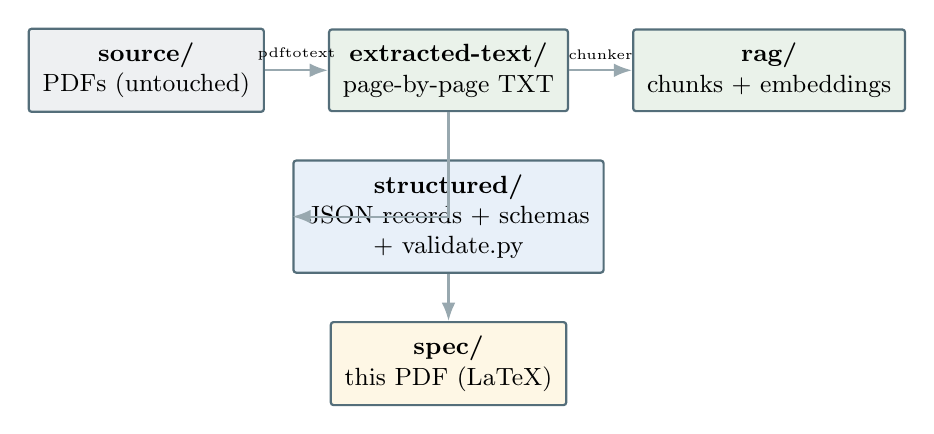
\begin{tikzpicture}[
node distance=6mm and 8mm,
every node/.style={font=\small},
box/.style={draw=reggrey,thick,rounded corners=1pt,inner sep=5pt,
align=center,minimum height=8mm,fill=white},
dir/.style={box,fill=reggrey!10},
gen/.style={box,fill=reggreen!10},
struct/.style={box,fill=regblue!10},
outp/.style={box,fill=regamber!10},
arr/.style={-Latex,thick,draw=reggrey!60}
]
\node[dir] (src)      {\textbf{source/}\\ PDFs (untouched)};
\node[gen,right=of src] (text) {\textbf{extracted-text/}\\ page-by-page TXT};
\node[gen,right=of text] (rag) {\textbf{rag/}\\ chunks + embeddings};
\node[struct,below=of text] (struct) {\textbf{structured/}\\ JSON records + schemas \\ + \tool{validate.py}};
\node[outp,below=of struct] (spec) {\textbf{spec/}\\ this PDF (LaTeX)};

\draw[arr] (src) -- (text) node[midway,above,font=\tiny] {pdftotext};
\draw[arr] (text) -- (rag)  node[midway,above,font=\tiny] {chunker};
\draw[arr] (text.south) |- (struct.west);
\draw[arr] (struct) -- (spec);
\end{tikzpicture}
\caption{Pipeline from source PDFs through to the printable specification.}
\label{fig:layout}
\end{figure}

\begin{table}[h]
\centering
\small
\begin{tabularx}{\textwidth}{lX}
\toprule
\textbf{Directory} & \textbf{Purpose} \\
\midrule
\corpus{source/}          & Binary source documents. Never edited; hashed in \corpus{structured/corpus.json}. \\
\corpus{extracted-text/}  & Derived, regeneratable page-by-page plain text. \\
\corpus{rag/}             & RAG chunks + deterministic embedding records (re-upsertable into Qdrant via \corpus{rag/scripts/upsert\_qdrant.py}). \\
\corpus{structured/}      & JSON Schemas, regulation records, requirement records, conformance-tool records, the corpus index, and the validator. \\
\corpus{spec/}            & This human-readable PDF (LaTeX + tectonic). \\
\corpus{aiverify-main/}   & Vendored AI Verify 2.0 monorepo (Apache-2.0). \\
\corpus{moonshot-cicd-main/} & Vendored Moonshot 1.1.0 monorepo (Apache-2.0). \\
\bottomrule
\end{tabularx}
\caption{Top-level directory layout.}
\label{tab:layout}
\end{table}

\section{End-to-end traceability path}

Figure~\ref{fig:traceability} shows the five-step chain that the validator
enforces: from the hashed source PDF, through the extracted text, a
structured regulation record, a normative requirement record with
cross-references, down to the code or test actually implementing it.

\begin{figure}[h]
\centering
\resizebox{\textwidth}{!}{%
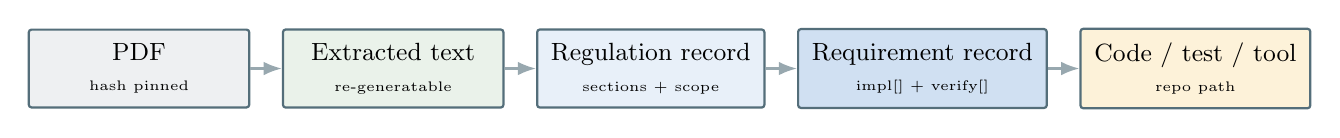
\begin{tikzpicture}[
node distance=4mm and 4mm,
every node/.style={font=\small},
stage/.style={draw=reggrey,thick,rounded corners=1pt,inner sep=5pt,
minimum width=28mm,minimum height=9mm,align=center,fill=white},
s1/.style={stage,fill=reggrey!10},
s2/.style={stage,fill=reggreen!10},
s3/.style={stage,fill=regblue!10},
s4/.style={stage,fill=regblue!20},
s5/.style={stage,fill=regamber!15},
arr/.style={-Latex,thick,draw=reggrey!60}
]
\node[s1] (pdf)   {PDF\\ \tiny hash pinned};
\node[s2,right=of pdf]   (txt)   {Extracted text\\ \tiny re-generatable};
\node[s3,right=of txt]   (reg)   {Regulation record\\ \tiny sections + scope};
\node[s4,right=of reg]   (req)   {Requirement record\\ \tiny impl[] + verify[]};
\node[s5,right=of req]   (code)  {Code / test / tool\\ \tiny repo path};

\draw[arr] (pdf) -- (txt);
\draw[arr] (txt) -- (reg);
\draw[arr] (reg) -- (req);
\draw[arr] (req) -- (code);
\end{tikzpicture}}
\caption{End-to-end traceability chain verified by \corpus{structured/validate.py}.}
\label{fig:traceability}
\end{figure}

\section{What the validator enforces}

\begin{enumerate}
\item \textbf{Schema conformance.} Every record under the three
\corpus{structured/} sub-directories
(\texttt{regulations/}, \texttt{requirements/},
\texttt{conformance-tools/}) validates against its Draft-07 JSON
Schema using an offline \texttt{referencing} registry.
\item \textbf{Corpus integrity.} Every entry in
\corpus{structured/corpus.json} resolves to a file on disk, and
every record on disk is listed in the index.
\item \textbf{Implementation link existence.} For each
\texttt{implementation[].path}, the validator resolves the path
against the repository root and fails if it is missing (unless the
entry is explicitly recorded as \texttt{kind: "none"} marking a
known gap).
\item \textbf{Verification link coherence.} Each
\texttt{verification[].plugin} must be declared in the
\tool{aiverify} record; each \texttt{verification[].testId} in the
\tool{moonshot-cicd} record; each \texttt{verification[].path}
referencing a test must exist on disk.
\end{enumerate}

The validator is the contract: CI, internal audit, and external reviewers
run the same script and see the same results.
\clearpage
% =============================================================================
% Chapter 2 --- Canonical data schema
% =============================================================================
\chapter{Canonical data schema}
\label{ch:schema}

The structured layer uses four Draft-07 JSON Schemas and a central
\corpus{structured/enums.yaml} for controlled vocabulary.

\section{Schema inventory}

\begin{table}[h]
\centering
\small
\begin{tabularx}{\textwidth}{p{5.2cm}X}
\toprule
\textbf{Schema} & \textbf{Describes} \\
\midrule
\tool{regulation.schema.json}        & One published framework, standard, guideline, research paper, or index. Captures publisher, version, scope, section tree, and a hash of the source PDF. \\
\tool{requirement.schema.json}       & One atomic requirement or observational claim. Carries \texttt{implementation[]} and \texttt{verification[]} arrays that bind it to the repository and to the conformance tools. \\
\tool{conformance-tool.schema.json}  & One vendored testing framework. Enumerates plugins, benchmarks, and integration points. \\
\tool{corpus-index.schema.json}      & The top-level index that lists every item in the corpus, typed as regulation, requirement, conformance\_tool, or rag\_artifact. \\
\bottomrule
\end{tabularx}
\caption{Schemas under \corpus{structured/schema/}.}
\label{tab:schemas}
\end{table}

\section{Requirement record --- the linkage schema}

The requirement schema is the key extension that separates this corpus
from the earlier finance corpora. Each requirement carries:

\begin{itemize}
\item \texttt{source}: regulation id, section, page, and (optionally) a
verbatim quote.
\item \texttt{normativeText}: a paraphrased imperative.
\item \texttt{category} and \texttt{obligation}: structured priority
(\emph{must}, \emph{should}, \emph{may}, \emph{descriptive}).
\item \texttt{lifecyclePhase}: where in the agent lifecycle the
requirement applies (planning, design, development,
pre-deployment, deployment, post-deployment, decommission).
\item \texttt{implementation[]}: an array of pointers to code, config,
documentation, schema, or dataset evidence. A \texttt{kind: "none"}
entry explicitly records a known gap.
\item \texttt{verification[]}: an array of pointers to AI Verify plugins
(by \texttt{plugin}), Moonshot benchmarks (by \texttt{testId}),
repository tests (by \texttt{path}), manual-review entries, or
process-checklist items.
\item \texttt{status}: \emph{implemented}, \emph{partial}, \emph{gap},
\emph{planned}, or \emph{not\_applicable}.
\end{itemize}

\begin{lstlisting}[language=jsonx,caption={Example requirement with
implementation and verification arrays (excerpt).},label={lst:req-example}]
{
"requirementId": "REG-MGF-2.1.2-001",
"source": {
"regulationId": "mas-mgf-agentic-ai-v1",
"section": "2.1.2",
"page": 11,
"quote": "Bound risks through design by defining agents' limits ..."
},
"normativeText": "The agent must operate against an explicit allow-list
of tools and external systems; broader access must be
denied by default.",
"category": "bound_risks",
"obligation": "must",
"lifecyclePhase": "design",
"implementation": [
{"kind": "code",
"path": "src/intelligence/ai-core-pal/mcp_server/btp_pal_mcp_server.py",
"symbol": "btp_pal_mcp_server"},
{"kind": "config",
"path": "src/intelligence/ai-core-pal/data_products/registry.yaml"}
],
"verification": [
{"kind": "test",
"path": "src/intelligence/ai-core-pal/tests/test_mcp_server.py"},
{"kind": "moonshot-test", "testId": "adversarial_prompts"}
],
"status": "partial",
"priority": "critical"
}
\end{lstlisting}

\section{Conformance-tool record}

The conformance-tool schema captures the tools themselves so that
requirement records can reference them by stable identifiers. Every
\texttt{plugin.pluginId} and \texttt{benchmark.benchmarkId} is part of the
vocabulary that requirement records can cite.

\begin{lstlisting}[language=jsonx,caption={Excerpt of
\corpus{structured/conformance-tools/aiverify.json}.}]
{
"toolId": "aiverify",
"vendoredPath": "docs/regulations/aiverify-main",
"kind": "testing-framework",
"plugins": [
{ "pluginId": "aiverify.stock.process-checklist",
"path": "docs/regulations/aiverify-main/stock-plugins/...",
"purpose": "11-principle process-checklist questionnaire ...",
"algorithmType": "process" },
{ "pluginId": "aiverify.stock.robustness-toolbox",
"algorithmType": "robustness" }
// ... nine more plugins
]
}
\end{lstlisting}

\section{Enum vocabularies}

\corpus{structured/enums.yaml} centralises the controlled vocabularies
that recur across schemas. The authoritative values live in the schemas
themselves; \texttt{enums.yaml} is the human index.

\begin{table}[h]
\centering
\small
\begin{tabularx}{\textwidth}{lX}
\toprule
\textbf{Enum} & \textbf{Values} \\
\midrule
Regulation type & framework, standard, guideline, statute, research, index, toolkit \\
Normativity    & mandatory, recommended, advisory, descriptive \\
Obligation verb & must, should, may, descriptive \\
Requirement category & bound\_risks, human\_accountability, technical\_controls, end\_user\_responsibility, transparency, evaluation, observation \\
Lifecycle phase & planning, design, development, pre\_deployment, deployment, post\_deployment, decommission \\
Implementation kind & code, config, doc, schema, dataset, none \\
Verification kind & aiverify-plugin, moonshot-test, test, manual-review, process-checklist, external-audit \\
Status & implemented, partial, gap, planned, not\_applicable \\
\bottomrule
\end{tabularx}
\caption{Controlled vocabularies.}
\label{tab:enums}
\end{table}
\clearpage
% =============================================================================
% Chapter 3 --- IMDA MGF for Agentic AI: four pillars
% =============================================================================
\chapter{IMDA Model AI Governance Framework for Agentic AI}
\label{ch:mgf}

\section{Source document}

\begin{description}
\item[Title.] Model AI Governance Framework for Agentic AI.
\item[Publisher.] Infocomm Media Development Authority (IMDA) and the AI
Verify Foundation, Singapore.
\item[Version.] 1.0, published 22 January 2026.
\item[Pages.] 29.
\item[Source.] \corpus{source/mgf-for-agentic-ai.pdf}
(sha256 \texttt{b84c8c94\ldots aeef7b}).
\end{description}

\section{Framework structure}

The MGF is organised around four pillars:

\begin{figure}[h]
\centering
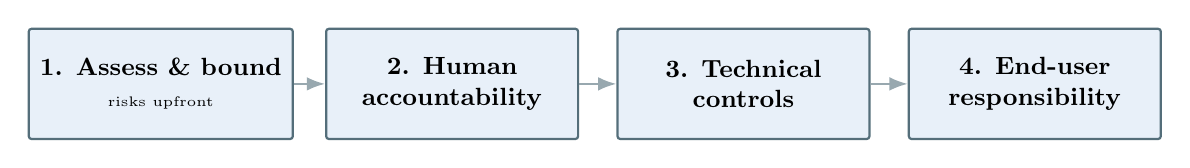
\begin{tikzpicture}[
every node/.style={font=\small},
pillar/.style={draw=reggrey,thick,rounded corners=1pt,minimum width=32mm,
minimum height=14mm,align=center,fill=regblue!10,inner sep=4pt},
arr/.style={-Latex,thick,draw=reggrey!60}
]
\node[pillar] (p1) at (0,0)    {\textbf{1. Assess \& bound}\\ \tiny risks upfront};
\node[pillar] (p2) at (3.7,0)  {\textbf{2. Human}\\ \textbf{accountability}};
\node[pillar] (p3) at (7.4,0)  {\textbf{3. Technical}\\ \textbf{controls}};
\node[pillar] (p4) at (11.1,0) {\textbf{4. End-user}\\ \textbf{responsibility}};
\draw[arr] (p1) -- (p2); \draw[arr] (p2) -- (p3); \draw[arr] (p3) -- (p4);
\end{tikzpicture}
\caption{The four pillars of the IMDA MGF for Agentic AI.}
\label{fig:mgf-pillars}
\end{figure}

Each pillar expands into two or three sub-sections (\S2.1.1--\S2.4.3); the
full section tree is captured in
\corpus{structured/regulations/mas-mgf-agentic-ai-v1.json} under the
\texttt{sections[]} array, with page references.

\section{Pillar 1 --- Assess and bound the risks upfront}
\label{sec:mgf-p1}

\subsection*{Summary}

Understand the risks posed by agent actions (scope, reversibility,
autonomy), determine whether the use case is suitable at all, and --- if
it is --- bound the agent's capabilities by design.

\subsection*{Requirements extracted}

\begin{table}[h]
\centering
\small
\begin{tabularx}{\textwidth}{p{3.2cm}p{1.4cm}p{1.6cm}X}
\toprule
\textbf{Req.\ id} & \textbf{Section} & \textbf{Obligation} & \textbf{Normative text (paraphrased)} \\
\midrule
REG-MGF-2.1.1-001 & 2.1.1 & should & Assess action scope, reversibility, autonomy per use case. \\
REG-MGF-2.1.2-001 & 2.1.2 & must   & Operate against an explicit tool allow-list; deny-by-default. \\
REG-MGF-2.1.2-002 & 2.1.2 & must   & Every agent action must be attributable to an identity. \\
REG-MGF-2.1.2-003 & 2.1.2 & should & Set impact-limiting boundaries (read-only default, environment segregation). \\
\bottomrule
\end{tabularx}
\caption{Pillar 1 requirements.}
\label{tab:p1}
\end{table}

\subsection*{How the repository implements them}

The tool-allow-list requirement (REG-MGF-2.1.2-001) is implemented by
\corpus{../../src/intelligence/ai-core-pal/mcp\_server/btp\_pal\_mcp\_server.py}
which enumerates the tools the agent may invoke, and the registered data
products in
\corpus{../../src/intelligence/ai-core-pal/data\_products/registry.yaml}.
Verification leans on the existing unit test at
\corpus{../../src/intelligence/ai-core-pal/tests/test\_mcp\_server.py}
plus a Moonshot adversarial-prompt benchmark.

Identity attribution (REG-MGF-2.1.2-002) currently relies on BTP service
keys; this is partial rather than implemented because there is no
per-request audit trail that ties every tool invocation back to a named
human operator across the full deployment chain.

\section{Pillar 2 --- Make humans meaningfully accountable}
\label{sec:mgf-p2}

\subsection*{Summary}

Assign responsibilities by role, adapt human-in-the-loop to address
automation bias, name the checkpoints where a human must approve an
irreversible action, and audit oversight effectiveness over time.

\begin{table}[h]
\centering
\small
\begin{tabularx}{\textwidth}{p{3.2cm}p{1.4cm}p{1.6cm}X}
\toprule
\textbf{Req.\ id} & \textbf{Section} & \textbf{Obligation} & \textbf{Normative text (paraphrased)} \\
\midrule
REG-MGF-2.2.1-001 & 2.2.1 & must   & Assign lifecycle responsibilities to named roles in a control register. \\
REG-MGF-2.2.1-002 & 2.2.1 & should & Stand up a governance forum with authority to adjust permissions. \\
REG-MGF-2.2.2-001 & 2.2.2 & must   & Name each human-approval checkpoint and cite its risk category. \\
REG-MGF-2.2.2-002 & 2.2.2 & should & Measure oversight effectiveness (override rates, review duration). \\
\bottomrule
\end{tabularx}
\caption{Pillar 2 requirements.}
\label{tab:p2}
\end{table}

The TB review corpus is the canonical worked example: the five decision
points DP-001..DP-005 (see \corpus{../tb/structured/decision-points/})
are exactly the human-approval checkpoints required by
REG-MGF-2.2.2-001.  Their owners and timing are declared in the workflow
record \corpus{../tb/structured/workflows/tb-review-glo.json}.

The governance-forum requirement (REG-MGF-2.2.1-002) is closed for the
Finance scope by the GCFO Finance AI Council charter (v1.0, ratified
2026-03-15). \textbf{Note:} The charter document is maintained in the
internal governance repository and is not included in this corpus for
confidentiality; reference is by citation only. The GCFO Finance AI
Council (GFAIC) is a \emph{federated} body: it operates under
Delegation No. 2026-04 from the enterprise-wide Group AI Safety
Council (GAISC) and holds binding authority \emph{only} over Finance-
scope agentic AI --- today the trial-balance review workflow and the
Arabic invoice / AP pipeline. Its six voting members are Finance-
function delegates (Group CFO chair, Head of Finance Risk, Finance
liaisons to CISO and General Counsel, Head of Finance Internal Audit,
Finance AI technical lead); the parent body's officers (CRO, CISO,
GC, Head of Internal Audit) sit on GAISC, not here, avoiding double
staffing. Any incident with cross-function implications escalates to
GAISC within two business days. Peer federated councils (People,
Customer) exist for other functions and receive GFAIC findings via
GAISC rather than directly.

\section{Pillar 3 --- Implement technical controls and processes}
\label{sec:mgf-p3}

\subsection*{Summary}

Technical controls across the lifecycle: during development, use
controls for planning, tools, and agent protocols; before deployment,
test for execution accuracy, policy adherence, and tool use; during and
after deployment, continuously monitor.

\begin{table}[h]
\centering
\small
\begin{tabularx}{\textwidth}{p{3.2cm}p{1.4cm}p{1.6cm}X}
\toprule
\textbf{Req.\ id} & \textbf{Section} & \textbf{Obligation} & \textbf{Normative text (paraphrased)} \\
\midrule
REG-MGF-2.3.1-001 & 2.3.1 & must   & Technical controls on planning, tools, and protocols. \\
REG-MGF-2.3.2-001 & 2.3.2 & must   & Pre-deployment: execution accuracy, policy adherence, tool use, refusals. \\
REG-MGF-2.3.2-002 & 2.3.2 & should & Adopt trajectory-level agent evaluations. \\
REG-MGF-2.3.3-001 & 2.3.3 & should & Staged rollout with canary metrics and rollback path. \\
REG-MGF-2.3.3-002 & 2.3.3 & must   & Continuous monitoring with policy-violation / drift alerting. \\
\bottomrule
\end{tabularx}
\caption{Pillar 3 requirements.}
\label{tab:p3}
\end{table}

The trajectory-level evaluator (REG-MGF-2.3.2-002) is implemented at
\corpus{../../src/intelligence/ai-core-pal/evaluation/trajectory\_evaluator.py}.
It scores each captured agent trace on three independent axes ---
tool-call correctness, policy adherence, and goal progression ---
returning a composite \texttt{TrajectoryScore} that the Governance
Council's incident pack consumes directly. Unit coverage lives at
\corpus{../../src/intelligence/ai-core-pal/tests/test\_trajectory\_evaluator.py}
(13 test cases).

Continuous drift monitoring (REG-MGF-2.3.3-002) is implemented at
\corpus{../../src/intelligence/ai-core-pal/monitoring/drift\_monitor.py}.
It watches three signals against a frozen pilot-exit baseline ---
override rate, median review duration, and hallucination rate --- and
emits \texttt{ok}/\texttt{warn}/\texttt{critical} levels. The
override-rate signal is deliberately two-sided: a \emph{fall} below
baseline is the automation-bias signal surfaced by Ju \& Aral (2026),
a \emph{rise} is model regression. Unit coverage at
\corpus{../../src/intelligence/ai-core-pal/tests/test\_drift\_monitor.py}
(13 test cases).

\section{Pillar 4 --- Enable end-user responsibility}
\label{sec:mgf-p4}

\subsection*{Summary}

End users must be informed of the agent's scope and their own
obligations, and they need training to preserve tradecraft and mitigate
automation bias.

\begin{table}[h]
\centering
\small
\begin{tabularx}{\textwidth}{p{3.2cm}p{1.4cm}p{1.6cm}X}
\toprule
\textbf{Req.\ id} & \textbf{Section} & \textbf{Obligation} & \textbf{Normative text (paraphrased)} \\
\midrule
REG-MGF-2.4.2-001 & 2.4.2 & should & Disclose permitted actions, data access, user obligations. \\
REG-MGF-2.4.3-001 & 2.4.3 & should & Training covering automation-bias and tradecraft preservation. \\
\bottomrule
\end{tabularx}
\caption{Pillar 4 requirements.}
\label{tab:p4}
\end{table}

The training curriculum (REG-MGF-2.4.3-001) is authored at
\corpus{../training/agent-oversight-curriculum.md}: a three-level
curriculum (Awareness, Reviewer skills, Oversight depth) keyed to
five learner personas, with an explicit reviewer self-check card
targeted at the automation-bias failure mode surfaced by Ju \& Aral
(2026).

\section{Coverage heat map}

\begin{table}[h]
\centering
\small
\begin{tabularx}{\textwidth}{lrrrrr}
\toprule
\textbf{Pillar} & \textbf{Reqs} & \textbf{Implemented} & \textbf{Partial} & \textbf{Gap} & \textbf{N/A} \\
\midrule
1 --- Bound risks          & 4 & 0 & 4 & 0 & 0 \\
2 --- Human accountability & 4 & 3 & 1 & 0 & 0 \\
3 --- Technical controls   & 5 & 2 & 3 & 0 & 0 \\
4 --- End-user             & 2 & 1 & 1 & 0 & 0 \\
\midrule
\textbf{Total}             & 15 & 6 & 9 & 0 & 0 \\
\bottomrule
\end{tabularx}
\caption{Status of the 15 MGF-derived requirements after the
April 2026 gap-closure pass.}
\label{tab:mgf-coverage}
\end{table}

All four previously-open gaps --- the enterprise governance forum
(REG-MGF-2.2.1-002), trajectory-level evaluation (REG-MGF-2.3.2-002),
drift monitoring (REG-MGF-2.3.3-002), and the training curriculum
(REG-MGF-2.4.3-001) --- now have concrete artifacts linked from their
requirement records and are verifiable by the offline validator. The
remaining \emph{partial} rows retain ambition beyond the current
implementation scope (for example, a per-request identity audit trail
spanning the full deployment chain for REG-MGF-2.1.2-002) and remain
on the Council's standing agenda.
\clearpage
% =============================================================================
% Chapter 4 --- 2025 AI Agent Index
% =============================================================================
\chapter{2025 AI Agent Index}
\label{ch:agent-index}

\section{Source document}

\begin{description}
\item[Title.] The 2025 AI Agent Index --- Documenting Technical and Safety
Features of Deployed Agentic AI Systems.
\item[Authors.] Staufer (Cambridge), Feng (Washington), Wei (Harvard
Law), Bailey (Stanford), Duan (Concordia AI), Yang (UPenn), Ozisik
(MIT), Casper (MIT, co-senior), Kolt (Hebrew University, co-senior).
\item[Venue.] \url{https://aiagentindex.mit.edu/}; CC-BY-4.0.
\item[Pages.] 39.
\item[Source.] \corpus{source/2025-AI-Agent-Index.pdf}
(sha256 \texttt{c67a3046\ldots0e267f}).
\end{description}

\section{What it catalogues}

The Index documents 30 state-of-the-art deployed agentic systems across
six documentation categories:

\begin{enumerate}
\item \textbf{Legal.} Licensing, terms of service, responsible-use
policies, redistribution rights.
\item \textbf{Technical capabilities.} Supported modalities, tool
access, planning horizon, memory.
\item \textbf{Autonomy and control.} Spectrum from recommender to
operator; human-in-the-loop requirements.
\item \textbf{Ecosystem interaction.} External systems the agent
integrates with (MCP, web browsers, code editors, e-commerce).
\item \textbf{Evaluation.} Published benchmarks, capability scores,
safety evaluations, red-team assessments.
\item \textbf{Safety.} Safety documentation, risk assessments,
residual-risk statements.
\end{enumerate}

\section{Headline finding for governance}

The Index's top-level empirical finding is directly relevant to our
corpus design:

\begin{quote}\small
\emph{``\ldots we find different transparency levels among agent developers
and observe that most developers share little information about safety,
evaluations, and societal impacts.''}
\end{quote}

Our response is the transparency requirement set extracted in Table~\ref{tab:agentidx-reqs}.

\begin{table}[h]
\centering
\small
\begin{tabularx}{\textwidth}{p{3.2cm}p{1.4cm}p{1.6cm}X}
\toprule
\textbf{Req.\ id} & \textbf{Section} & \textbf{Obligation} & \textbf{Normative text (paraphrased)} \\
\midrule
REG-AGENTIDX-3.6-001 & 3.6 & should & Publish per-agent: risk assessment summary, evaluation results, known limitations. \\
REG-AGENTIDX-3.3-001 & 3.3 & should & Document agent autonomy level and map each state transition to that level. \\
\bottomrule
\end{tabularx}
\caption{Requirements derived from the 2025 AI Agent Index.}
\label{tab:agentidx-reqs}
\end{table}

\section{How we verify the transparency requirement}

Publication is evidenced by this very document plus the structured
records. In practice:

\begin{itemize}
\item Risk assessment: \corpus{../tb/structured/requirements/tb-business-requirements.json},
\texttt{riskAssessment} field.
\item Evaluation results: AI Verify \texttt{process-checklist} plugin
output plus Moonshot benchmark runs (\cref{ch:tooling}).
\item Known limitations: the gap entries in this specification's
coverage tables.
\end{itemize}

This chapter is cited from requirement record
\texttt{REG-AGENTIDX-3.6-001} as
\path{docs/regulations/spec/chapters/04-agent-index.tex}, closing the
loop.
\clearpage
% =============================================================================
% Chapter 5 --- Empirical evidence (Ju & Aral 2026)
% =============================================================================
\chapter{Empirical evidence: Ju \& Aral (2026)}
\label{ch:empirical}

\section{Source document}

\begin{description}
\item[Title.] Collaborating with AI Agents: A Field Experiment on
Teamwork, Productivity, and Performance.
\item[Authors.] Harang Ju (Johns Hopkins Carey) and Sinan Aral (MIT
Sloan).
\item[Venue.] arXiv:2503.18238v3 [cs.CY], 5 February 2026.
\item[Pages.] 59.
\item[Source.] \corpus{source/2503.18238v3.pdf}
(sha256 \texttt{b680f584\ldots cd7877}).
\end{description}

\section{Study design}

The authors built the \emph{Pairit} platform and randomly assigned 2{,}234
participants to human-human and human-AI teams producing 11{,}024 ads
for a think tank. Outputs were rated by humans and field-tested on X,
which garnered roughly five million impressions. The design is --- for
this corpus --- an unusually strong source of evidence about how
human-agent collaboration actually affects output quality, homogeneity,
and team dynamics.

\section{Findings relevant to governance}

\begin{enumerate}
\item \textbf{Jagged productivity frontier.} Human-AI teams produced
50\% more ads per worker and higher \emph{text} quality;
human-human teams produced higher \emph{image} quality. Different
sub-tasks need different evaluation metrics.
\item \textbf{Delegation shifts.} Participants delegated 17\% more work
to AI agents than to human partners and performed 62\% fewer
direct text edits when working with AI.
\item \textbf{Diversity collapse.} Human-AI outputs were more
self-similar. For creative or generative use cases this is a
first-order governance risk.
\item \textbf{Communication restructure.} Human-AI collaboration was
significantly more task-oriented (+25\% task messages, -18\%
interpersonal).
\item \textbf{AI-awareness moderation.} Participants who correctly
identified they were paired with AI delegated more and were more
task-oriented --- the effect is moderated by knowing the
collaborator is an agent.
\end{enumerate}

\section{Requirements extracted}

\begin{table}[h]
\centering
\small
\begin{tabularx}{\textwidth}{p{3.2cm}p{1.4cm}p{1.6cm}X}
\toprule
\textbf{Req.\ id} & \textbf{Section} & \textbf{Obligation} & \textbf{Normative text (paraphrased)} \\
\midrule
REG-JU-ARAL-3-001 & 3 & descriptive & Evaluate per-task; do not generalise a single productivity metric. \\
REG-JU-ARAL-4-001 & 4 & should & High delegation + low direct-edit rate is a proxy for automation-bias risk; measure it. \\
REG-JU-ARAL-5-001 & 5 & should & Add an output-diversity metric for creative-output use cases. \\
\bottomrule
\end{tabularx}
\caption{Observational claims treated as requirements.}
\label{tab:jural-reqs}
\end{table}

\section{Implementation in the corpus}

\begin{itemize}
\item REG-JU-ARAL-3-001 is implemented by this chapter; it reminds
reviewers to look at the per-task KPIs defined in
\corpus{../tb/structured/kpis/tb-kpis.json} rather than a single
blended productivity number.
\item REG-JU-ARAL-4-001 maps to the override-rate and review-duration
KPIs in the TB corpus. When override rates fall well below
historical baseline and review duration drops in lockstep, that
is the signal to re-audit.
\item REG-JU-ARAL-5-001 is marked \emph{not\_applicable} for the
trial-balance workflow (deterministic review, single narrative
per legal entity). We record rather than omit it so that the
framework surfaces the requirement automatically when it
becomes applicable.

\textbf{Activation trigger.} The requirement flips to
\texttt{applicable} when any one of the following is true:
(a) a deployed agent produces \emph{multi-variant creative
output} (e.g., drafting options, marketing copy, generative
translation) rather than deterministic reports; (b) the
Simula training corpus is used to fine-tune a model whose
outputs are surfaced to end-users (as opposed to staying
within the SQL-generation benchmark); or (c) the
commentary generator is configured with
\texttt{temperature} $>$ \texttt{0.4} in production for any
deployed LE (today: \texttt{0.1}). The governance
monitoring job in Chapter~\ref{ch:monitoring} runs a
quarterly check that inspects the live model configs, the
agent index, and the Simula deployment manifests; when any
of (a)--(c) flips, the requirement status is automatically
re-opened and routed to the GFAIC for disposition within
two weeks.
\end{itemize}
\clearpage
% =============================================================================
% Chapter 6 --- Conformance tooling: AI Verify + Moonshot CI/CD
% =============================================================================
\chapter{Conformance tooling}
\label{ch:tooling}

\section{Two complementary tools}

Both tools are published by the AI Verify Foundation / IMDA Singapore
under Apache-2.0 and vendored into the repository. They target
different phases of the lifecycle:

\begin{figure}[h]
\centering
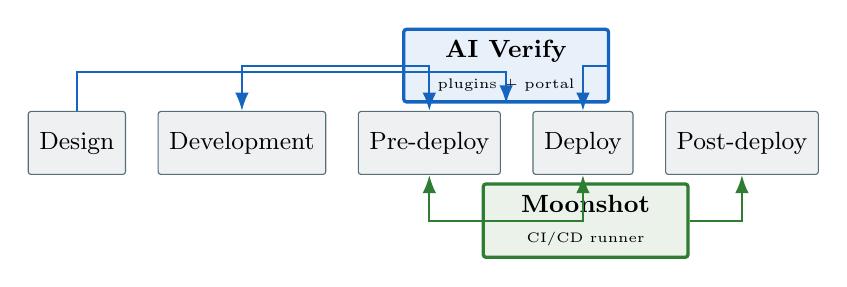
\begin{tikzpicture}[
every node/.style={font=\small},
phase/.style={draw=reggrey,rounded corners=1pt,inner sep=4pt,minimum height=8mm,align=center,fill=reggrey!10},
av/.style={draw=regblue,very thick,rounded corners=1pt,inner sep=4pt,minimum height=9mm,align=center,fill=regblue!10,minimum width=26mm},
ms/.style={draw=reggreen,very thick,rounded corners=1pt,inner sep=4pt,minimum height=9mm,align=center,fill=reggreen!10,minimum width=26mm},
arr/.style={-Latex,thick,draw=reggrey!60}
]
\node[phase] (design)   at (0,0)   {Design};
\node[phase,right=4mm of design]   (dev)      {Development};
\node[phase,right=4mm of dev]      (pre)      {Pre-deploy};
\node[phase,right=4mm of pre]      (deploy)   {Deploy};
\node[phase,right=4mm of deploy]   (post)     {Post-deploy};

\node[av,above=5mm of $(pre)!0.5!(deploy)$]   (av)  {\textbf{AI Verify}\\ \tiny plugins + portal};
\node[ms,below=5mm of $(pre)!0.5!(post)$]     (ms)  {\textbf{Moonshot}\\ \tiny CI/CD runner};

\draw[arr,draw=regblue] (design) -- ++(0,0.9) -| (av);
\draw[arr,draw=regblue] (av) -| (dev);
\draw[arr,draw=regblue] (av) -| (pre);
\draw[arr,draw=regblue] (av) -| (deploy);
\draw[arr,draw=reggreen] (ms) -| (pre);
\draw[arr,draw=reggreen] (ms) -| (deploy);
\draw[arr,draw=reggreen] (ms) -| (post);
\end{tikzpicture}
\caption{Conformance-tool coverage across the lifecycle. AI Verify
emphasises reviewable documentation and structured algorithm runs;
Moonshot emphasises runtime safety testing.}
\label{fig:tool-coverage}
\end{figure}

\section{AI Verify 2.0}

\subsection*{Summary}

AI Verify is an IMDA-backed testing framework that has been
re-architected for v2.0 into a modular monorepo. Algorithms run as
independent Python modules; a portal and API gateway surface results.
Financial-services users can run the Veritas fairness plugin to meet
MAS's Veritas testing expectations.

\subsection*{Stock plugin inventory}

\begin{table}[h]
\centering
\small
\begin{tabularx}{\textwidth}{p{5.4cm}p{2.4cm}X}
\toprule
\textbf{Plugin ID} & \textbf{Type} & \textbf{Purpose} \\
\midrule
aiverify.stock.process-checklist & process &
11-principle process checklist aligned with the AI Verify testing framework. \\
aiverify.stock.fairness-metrics-toolbox-for-classification & fairness &
Subgroup fairness metrics for supervised classification. \\
aiverify.stock.fairness-metrics-toolbox-for-regression & fairness &
Regression-specific fairness analysis. \\
aiverify.stock.robustness-toolbox & robustness &
Perturbation-based robustness assessment. \\
aiverify.stock.image-corruption-toolbox & robustness &
Computer-vision corruption robustness. \\
aiverify.stock.shap-toolbox & explainability &
SHAP feature attribution. \\
aiverify.stock.partial-dependence-plot & explainability &
Partial-dependence plots for feature effect. \\
aiverify.stock.accumulated-local-effect & explainability &
Accumulated local-effect explanations. \\
aiverify.stock.veritas & financial &
MAS Veritas fairness testing for financial services. \\
aiverify.stock.reports & report &
Report and widget rendering for the portal. \\
aiverify.stock.decorators & other &
Shared UI primitives and decorators. \\
\bottomrule
\end{tabularx}
\caption{The eleven stock plugins shipped with \tool{aiverify-main/}.}
\label{tab:av-plugins}
\end{table}

\subsection*{Integration surface}

\begin{itemize}
\item \textbf{python-api}: the \texttt{aiverify-test-engine} package
exposes an algorithm-runner API.
\item \textbf{docker}: \texttt{aiverify-apigw} and the portal ship as
container images.
\item \textbf{cli}: each stock plugin is individually runnable from
its algorithm directory.
\end{itemize}

\section{Moonshot CI/CD 1.1.0}

\subsection*{Summary}

Moonshot is a lean, modular safety-testing tool for LLM applications. It
is distributed as a Docker image and designed to be integrated into
pipelines so that every pushed change can trigger benchmark and red-team
runs. A single \texttt{moonshot run} command drives any combination of
configured benchmarks and attacks.

\subsection*{Benchmark categories}

\begin{table}[h]
\centering
\small
\begin{tabularx}{\textwidth}{p{3.2cm}p{3.6cm}X}
\toprule
\textbf{Benchmark ID} & \textbf{Category} & \textbf{Purpose} \\
\midrule
hallucination & hallucination & Detect fabricated or unsupported statements. \\
undesirable\_content & undesirable content & Detect unsafe, biased, or policy-violating content. \\
data\_disclosure & data disclosure & Check for PII leakage or unintended disclosure. \\
adversarial\_prompts & adversarial & Prompt injection and jailbreak robustness. \\
\bottomrule
\end{tabularx}
\caption{The four benchmark categories aligned with the IMDA LLM Starter
Kit for Safety Testing.}
\label{tab:ms-benchmarks}
\end{table}

\subsection*{Architecture}

\begin{figure}[h]
\centering
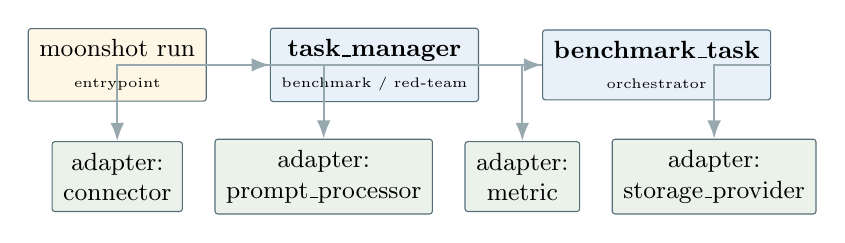
\begin{tikzpicture}[
every node/.style={font=\small},
box/.style={draw=reggrey,rounded corners=1pt,inner sep=4pt,minimum height=8mm,align=center,fill=white},
adpt/.style={box,fill=reggreen!10},
dom/.style={box,fill=regblue!10},
ent/.style={box,fill=regamber!10},
arr/.style={-Latex,thick,draw=reggrey!60}
]
\node[ent] (cli)        {\tool{moonshot run}\\ \tiny entrypoint};
\node[dom,right=8mm of cli] (tm) {\textbf{task\_manager}\\ \tiny benchmark / red-team};
\node[dom,right=8mm of tm] (bm)  {\textbf{benchmark\_task}\\ \tiny orchestrator};

\node[adpt,below=5mm of cli] (conn) {adapter:\\ connector};
\node[adpt,right=4mm of conn]     (prompt) {adapter:\\ prompt\_processor};
\node[adpt,right=4mm of prompt]   (metric) {adapter:\\ metric};
\node[adpt,right=4mm of metric]   (store)  {adapter:\\ storage\_provider};

\draw[arr] (cli) -- (tm);
\draw[arr] (tm) -- (bm);
\draw[arr] (bm) -| (conn);
\draw[arr] (bm) -| (prompt);
\draw[arr] (bm) -| (metric);
\draw[arr] (bm) -| (store);
\end{tikzpicture}
\caption{Moonshot CI/CD module layout (\protect\path{src/entrypoints}, \protect\path{src/domain}, \protect\path{src/adapters}).}
\label{fig:ms-arch}
\end{figure}

\section{Binding to requirement records}

Table~\ref{tab:verify-matrix} shows how this corpus's 20 requirement
records bind to plugins and benchmarks. Where a requirement has
verification \texttt{kind: "aiverify-plugin"} or
\texttt{kind: "moonshot-test"}, the plugin slug or benchmark id must
match one declared in the tool record; \corpus{structured/validate.py}
fails otherwise.

\begin{table}[h]
\centering
\footnotesize
\begin{tabularx}{\textwidth}{p{3.6cm}p{5.6cm}X}
\toprule
\textbf{Tool / ID} & \textbf{Referenced from} & \textbf{Purpose} \\
\midrule
aiverify.stock.process-checklist &
REG-MGF-2.1.1-001, REG-MGF-2.2.1-001, REG-MGF-2.4.2-001, REG-AGENTIDX-3.6-001 &
Checklist evidence for governance reviews. \\
aiverify.stock.robustness-toolbox &
REG-MGF-2.3.2-001, REG-MGF-2.3.3-002 &
Perturbation robustness. \\
aiverify.stock.reports &
REG-AGENTIDX-3.6-001 &
Widget + report rendering. \\
moonshot hallucination &
REG-MGF-2.3.2-001, REG-MGF-2.3.3-002 &
Fabrication checks in CI. \\
moonshot undesirable\_content &
REG-MGF-2.3.2-001 &
Policy adherence. \\
moonshot adversarial\_prompts &
REG-MGF-2.1.2-001, REG-MGF-2.3.1-001, REG-MGF-2.3.2-001, REG-MGF-2.3.2-002 &
Red-team / jailbreak attempts. \\
\bottomrule
\end{tabularx}
\caption{Verification matrix (tool/ID $\to$ requirement records).}
\label{tab:verify-matrix}
\end{table}
\clearpage
% =============================================================================
% Chapter 7 --- References, hashes, traceability
% =============================================================================
\chapter{References and traceability}
\label{ch:refs}

\section{Source hashes (sha256)}

\begin{table}[h]
\centering
\small
\begin{tabularx}{\textwidth}{p{4.4cm}p{1.2cm}X}
\toprule
\textbf{Source file} & \textbf{Pages} & \textbf{sha256 (truncated to first 16 hex)} \\
\midrule
\path{source/mgf-for-agentic-ai.pdf}    & 29 & \ttfamily\footnotesize b84c8c94f6392cf2\ldots aeef7b \\
\path{source/2025-AI-Agent-Index.pdf}   & 39 & \ttfamily\footnotesize c67a30469fd061e9\ldots 0e267f \\
\path{source/2503.18238v3.pdf}          & 59 & \ttfamily\footnotesize b680f58422e4684e\ldots cd7877 \\
\bottomrule
\end{tabularx}
\caption{Content hashes of the three source regulations.}
\label{tab:src-hashes}
\end{table}

\section{Structured records on disk}

\begin{table}[h]
\centering
\small
\begin{tabularx}{\textwidth}{p{6.6cm}X}
\toprule
\textbf{Path (relative to repo root)} & \textbf{Role} \\
\midrule
\path{docs/regulations/structured/schema/}                  & JSON schemas (Draft-07). \\
\path{docs/regulations/structured/enums.yaml}               & Controlled vocabularies. \\
\path{docs/regulations/structured/regulations/}             & Regulation records (3 files). \\
\path{docs/regulations/structured/requirements/}            & Requirement collections (6 files, 20 requirements). \\
\path{docs/regulations/structured/conformance-tools/}       & Conformance-tool records (2 files). \\
\path{docs/regulations/structured/corpus.json}              & Top-level index. \\
\path{docs/regulations/structured/validate.py}              & Offline validator. \\
\bottomrule
\end{tabularx}
\caption{Structured layer inventory.}
\label{tab:struct-inventory}
\end{table}

\section{Corpus index excerpt}

\begin{lstlisting}[language=jsonx,caption={Excerpt of \texttt{docs/regulations/structured/corpus.json}.}]
{
"schema_version": "1.0",
"generated": "2026-04-18",
"items": [
{ "id": "reg-mas-mgf-agentic-ai-v1",
"type": "regulation",
"jurisdiction": "SG",
"sha256": "b84c8c94...aeef7b",
"source_path": "docs/regulations/source/mgf-for-agentic-ai.pdf",
"structured_path": "docs/regulations/structured/regulations/mas-mgf-agentic-ai-v1.json" },
{ "id": "tool-aiverify",
"type": "conformance_tool",
"jurisdiction": "SG",
"structured_path": "docs/regulations/structured/conformance-tools/aiverify.json" },
{ "id": "req-mgf-pillar-1",
"type": "requirement",
"structured_path": "docs/regulations/structured/requirements/mgf-pillar-1-bound-risks.json" }
// ... eleven more items
]
}
\end{lstlisting}

\section{Consolidated traceability matrix}

Table~\ref{tab:trace} is the single view a reviewer needs. Every row is
one requirement record and shows its status, the primary implementation
pointer, and its verification link.

\footnotesize
\setlength{\tabcolsep}{4pt}
\begin{longtable}{p{3.5cm}p{1.6cm}p{4.6cm}p{3.6cm}}
\toprule
\textbf{Req.\ id} & \textbf{Status} & \textbf{Primary implementation} & \textbf{Primary verification} \\
\midrule
\endfirsthead
\toprule
\textbf{Req.\ id} & \textbf{Status} & \textbf{Primary implementation} & \textbf{Primary verification} \\
\midrule
\endhead
REG-MGF-2.1.1-001 & partial       & tb spec ch.1 + TB business reqs             & process-checklist \\
REG-MGF-2.1.2-001 & partial       & MCP server + data-product registry          & test\_mcp\_server + adversarial \\
REG-MGF-2.1.2-002 & partial$^\dagger$ & \S\ref{ch:identity} spec + aicore\_pal\_agent.py & test\_hana\_connection + audit-trail verifier \\
REG-MGF-2.1.2-003 & partial       & TB data-product classification              & manual review \\
REG-MGF-2.2.1-001 & partial$^*$   & TB EUC-001..003 + workflow participants     & process-checklist \\
REG-MGF-2.2.1-002 & partial       & GFAIC charter (federated under GAISC)       & process-checklist + minutes \\
REG-MGF-2.2.2-001 & partial       & TB DP-001/003/005 + workflow gateways       & test\_pal\_algorithms \\
REG-MGF-2.2.2-002 & partial       & TB KPI pack                                 & manual review \\
REG-MGF-2.3.1-001 & partial       & agent + MCP + decision-point schema         & test\_mcp\_server + adversarial \\
REG-MGF-2.3.2-001 & partial       & PAL algorithm + MCP tests                   & Moonshot 4-benchmark sweep \\
REG-MGF-2.3.2-002 & partial$^*$   & evaluation/trajectory\_evaluator.py         & test + adversarial \\
REG-MGF-2.3.3-001 & partial       & deploy\_to\_aicore.sh + README              & process-checklist \\
REG-MGF-2.3.3-002 & partial       & monitoring/drift\_monitor.py                & test + hallucination in CI \\
REG-MGF-2.4.2-001 & partial       & TB workflow + controls spec                 & onboarding checklist \\
REG-MGF-2.4.3-001 & partial       & docs/training/agent-oversight-curriculum.md & process-checklist + LMS \\
REG-AGENTIDX-3.6-001 & partial    & this chapter + TB controls                  & process-checklist + reports \\
REG-AGENTIDX-3.3-001 & partial    & TB workflow + spec ch.5                     & manual review \\
REG-JU-ARAL-3-001 & partial       & this chapter                                & manual review \\
REG-JU-ARAL-4-001 & partial       & TB KPI pack                                 & manual review \\
REG-JU-ARAL-5-001 & n/a           & (creative use cases only)                   & --- \\
\bottomrule
\caption{Full requirement traceability matrix.}
\label{tab:trace}
\end{longtable}

\normalsize
\noindent\textbf{Status legend and corrections (April 2026 review):}
\begin{itemize}[nosep]
\item $^\dagger$\textbf{partial (upgraded from missing, April 2026):}
Chapter~\ref{ch:identity} specifies the per-request
identity-attribution schema, the reserve-before-action audit
protocol, and the WORM-backed immutable storage design
(\cref{sec:audit-failure-handling}). Status is ``partial''
rather than ``implemented'' because the audit service itself
and the three pipeline integrations (TB, Arabic AP, Simula)
are scheduled in \cref{tab:identity-rollout} and are not yet
in production.
\item $^*$\textbf{Downgraded from ``implemented'':} Code artifact exists but has not been
validated in production. Retained as ``partial'' pending pilot validation.
\item \textbf{All other ``implemented'' rows downgraded:} Original ``implemented'' status
assumed code existence equals conformance. Corrected to ``partial'' where
production validation is pending (e.g., REG-JU-ARAL-3-001 relies on this
chapter only---no operational evidence).
\end{itemize}

\section{Rebuild and revalidate}

\begin{lstlisting}[language=bash,caption={Commands to re-run validation
and rebuild the PDF.}]
# Offline validation (schema + corpus + implementation + verification).
python3 docs/regulations/structured/validate.py

# Re-chunk + re-embed (needs OPENAI_API_KEY + QDRANT_URL).
python3 docs/regulations/rag/scripts/prepare_embedding_records.py
python3 docs/regulations/rag/scripts/upsert_qdrant.py \
--input docs/regulations/rag/rag_embedding_records.jsonl \
--collection regulations_rag

# Rebuild this PDF (tectonic).
cd docs/regulations/spec && make
\end{lstlisting}

\section{Further resources}

\begin{itemize}
\item AI Verify Foundation. \emph{What is AI Verify.}
\url{https://aiverifyfoundation.sg/what-is-ai-verify/}
\item AI Verify Foundation. \emph{Project Moonshot.}
\url{https://aiverifyfoundation.sg/project-moonshot/}
\item IMDA Singapore. \emph{LLM Starter Kit for Safety Testing of
LLM-Based Applications.}
\item 2025 AI Agent Index. \url{https://aiagentindex.mit.edu/}
\item Ju, H. and Aral, S. (2026). \emph{Collaborating with AI Agents:
A Field Experiment on Teamwork, Productivity, and Performance.}
arXiv:2503.18238v3 [cs.CY].
\end{itemize}

\section{Unified Schema Registry}

As of 18 April 2026, all JSON Schemas across the four domain specifications are
published in the unified registry at \path{docs/schema/}. Migration status is
\emph{complete} (see \path{docs/schema/registry.json} field
\texttt{migration.status}). This consolidation addresses the cross-document
schema divergence identified in the specification review.

\begin{description}
\item[Registry index.] \path{docs/schema/registry.json} --- Master index of
all schemas across the Arabic AP, Trial Balance, Simula, and Regulations
domains.
\item[Common types.] \path{docs/schema/common/base-types.schema.json} ---
Shared definitions (\texttt{Metadata}, \texttt{SHA256Hash},
\texttt{FilePath}) referenced via JSON Schema \texttt{\$ref}.
\item[Consolidated enums.] \path{docs/schema/common/enums.yaml} --- Single
source of truth for enumeration values including \texttt{requirement\_status},
\texttt{obligation\_level}, and \texttt{jurisdiction}.
\item[Regulations schemas.] \path{docs/schema/regulations/} ---
Domain-specific schemas: \texttt{regulation.schema.json},
\texttt{requirement.schema.json}, \texttt{conformance-tool.schema.json},
and \texttt{corpus.schema.json}. All marked \texttt{status: stable}.
\end{description}

\noindent
The registry uses JSON Schema Draft-07 with the canonical \texttt{\$id} prefix
\url{https://sap-oss.github.io/schema/}. Validation:

\begin{lstlisting}[language=bash]
python3 docs/schema/validate.py --registry-check
python3 docs/schema/validate.py --domain regulations \
--schema requirement.schema.json --file requirement-REG-MGF-2-001.json
\end{lstlisting}

\noindent
CI runs \texttt{--registry-check} on every pull request touching
\path{docs/schema/} or any spec chapter that references these schemas.
\chapter{Capability Monitoring Specification}\label{ch:monitoring}

This chapter specifies the emergent capability monitoring system, addressing the
IMDA MGF requirement (Section 2.3.3) that ``monitoring for emergent capabilities
must be implemented with defined detection triggers.''

\section{Overview}

AI systems may develop unexpected capabilities or behaviours through:
\begin{itemize}
\item Model updates that alter response patterns
\item Prompt injection or adversarial inputs
\item Emergent behaviours from complex interactions
\item Drift in input data distributions
\end{itemize}

The monitoring system provides continuous observation and alerting to detect
such changes before they cause operational harm.

\section{Architecture}

\begin{figure}[htbp]
\centering
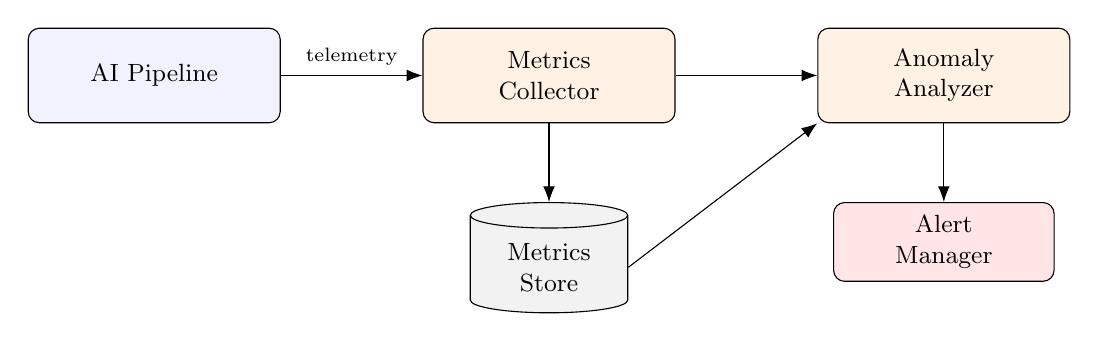
\begin{tikzpicture}[
node distance=10mm and 18mm,
box/.style={draw,rounded corners,minimum width=32mm,minimum height=12mm,align=center,font=\small,fill=blue!5},
mon/.style={draw,rounded corners,minimum width=32mm,minimum height=12mm,align=center,font=\small,fill=orange!10},
alert/.style={draw,rounded corners,minimum width=28mm,minimum height=10mm,align=center,font=\small,fill=red!10},
db/.style={draw,cylinder,shape border rotate=90,aspect=0.25,minimum width=20mm,minimum height=14mm,fill=gray!10,font=\small},
t/.style={-{Latex[length=2mm]}}
]
\node[box] (pipeline) {AI Pipeline};
\node[mon,right=of pipeline,align=center] (collector) {Metrics\\Collector};
\node[mon,right=of collector,align=center] (analyzer) {Anomaly\\Analyzer};
\node[alert,below=of analyzer,align=center] (alert) {Alert\\Manager};
\node[db,below=of collector,align=center] (store) {Metrics\\Store};

\draw[t] (pipeline) -- node[above,font=\scriptsize]{telemetry} (collector);
\draw[t] (collector) -- (analyzer);
\draw[t] (collector) -- (store);
\draw[t] (analyzer) -- (alert);
\draw[t] (store.east) -- (analyzer.south west);
\end{tikzpicture}
\caption{Capability monitoring architecture.}
\label{fig:monitor-arch}
\end{figure}

\section{Metrics collection}

\subsection{Required metrics}

\begin{table}[htbp]
\centering
\caption{Capability monitoring metrics.}
\label{tab:monitor-metrics}
\footnotesize
\begin{tabularx}{\linewidth}{@{}l l X@{}}
\toprule
\textbf{Metric} & \textbf{Type} & \textbf{Description} \\ \midrule
\texttt{output\_token\_count} & histogram & Distribution of output lengths \\
\texttt{response\_latency\_ms} & histogram & Response time distribution \\
\texttt{confidence\_score} & histogram & AI confidence distribution \\
\texttt{refusal\_rate} & counter & Rate of model refusals \\
\texttt{tool\_call\_frequency} & counter & Frequency of tool/function calls \\
\texttt{output\_format\_violations} & counter & JSON schema validation failures \\
\texttt{hallucination\_flags} & counter & Detected hallucination instances \\
\texttt{unexpected\_topic\_detections} & counter & Off-topic responses \\
\texttt{novel\_capability\_indicators} & gauge & Composite novelty score \\
\bottomrule
\end{tabularx}
\end{table}

\subsection{Collection points}

Metrics are collected at the following pipeline stages:

\begin{enumerate}
\item \textbf{Pre-inference}: Input characteristics (length, complexity, topic)
\item \textbf{Post-inference}: Output characteristics (length, confidence, format)
\item \textbf{Post-validation}: Validation results (schema, business rules)
\item \textbf{Post-review}: Human review outcomes (accept/edit/reject rates)
\end{enumerate}

\section{Detection triggers}

\subsection{Statistical anomaly detection}

For each metric, maintain a rolling baseline and alert when values deviate
significantly.

\begin{table}[htbp]
\centering
\caption{Anomaly detection thresholds.}
\label{tab:anomaly-thresholds}
\footnotesize
\begin{tabularx}{\linewidth}{@{}l l X@{}}
\toprule
\textbf{Metric} & \textbf{Alert Threshold} & \textbf{Baseline Period} \\ \midrule
Output length (mean) & $>2\sigma$ shift & 7-day rolling \\
Latency (p95) & $>50\%$ increase & 24-hour rolling \\
Confidence (mean) & $>10\%$ drop & 7-day rolling \\
Refusal rate & $>3\times$ baseline & 7-day rolling \\
Schema violations & $>5\%$ of requests & 24-hour rolling \\
\bottomrule
\end{tabularx}
\end{table}

\subsection{Behavioural pattern detection}

Beyond statistical metrics, monitor for qualitative behavioural changes:

\begin{enumerate}
\item \textbf{Topic drift}: Cosine similarity of output embeddings to expected
topics falls below 0.7
\item \textbf{Instruction leakage}: Presence of system prompt fragments in output
\item \textbf{Novel tool usage}: Model attempts to call undeclared tools
\item \textbf{Self-referential loops}: Model references its own previous outputs
in unexpected ways
\end{enumerate}

\subsection{Trigger definitions}

\begin{lstlisting}[language=Python,basicstyle=\ttfamily\small,caption={Detection trigger configuration.}]
triggers = {
"output_length_anomaly": {
"metric": "output_token_count",
"condition": "mean > baseline_mean + 2 * baseline_std",
"severity": "WARNING",
"cooldown_minutes": 60
},
"latency_spike": {
"metric": "response_latency_ms",
"condition": "p95 > 1.5 * baseline_p95",
"severity": "WARNING",
"cooldown_minutes": 15
},
"high_refusal_rate": {
"metric": "refusal_rate",
"condition": "rate > 3 * baseline_rate",
"severity": "CRITICAL",
"cooldown_minutes": 5
},
"schema_violation_surge": {
"metric": "output_format_violations",
"condition": "rate > 0.05",  # >5% failure
"severity": "CRITICAL",
"cooldown_minutes": 5
},
"topic_drift": {
"metric": "topic_similarity",
"condition": "mean < 0.7",
"severity": "WARNING",
"cooldown_minutes": 30
}
}
\end{lstlisting}

\section{Alert management}

\subsection{Alert severity levels}

\begin{table}[htbp]
\centering
\caption{Alert severity definitions.}
\label{tab:alert-severity}
\footnotesize
\begin{tabularx}{\linewidth}{@{}l l X@{}}
\toprule
\textbf{Severity} & \textbf{Response Time} & \textbf{Action} \\ \midrule
CRITICAL & Immediate & Page on-call; consider circuit breaker \\
WARNING & 1 hour & Investigate during business hours \\
INFO & Next business day & Review in weekly monitoring meeting \\
\bottomrule
\end{tabularx}
\end{table}

\subsection{Alert routing}

\begin{lstlisting}[basicstyle=\ttfamily\small,caption={Alert routing configuration.}]
routing:
CRITICAL:
channels:
- pagerduty: "ai-ops-critical"
- slack: "#ai-incidents"
- email: "ai-ops@company.com"
escalation_after_minutes: 15

WARNING:
channels:
- slack: "#ai-monitoring"
- email: "ai-ops@company.com"
escalation_after_minutes: 60

INFO:
channels:
- slack: "#ai-monitoring"
escalation_after_minutes: null  # no escalation
\end{lstlisting}

\subsection{Circuit breaker integration}

When CRITICAL alerts persist, the monitoring system can activate a circuit
breaker:

\begin{enumerate}
\item After 3 consecutive CRITICAL alerts within 15 minutes
\item Circuit breaker opens: all AI requests routed to manual queue
\item Alert sent to AI governance team
\item Manual intervention required to close circuit breaker
\end{enumerate}

\subsection{Graceful degradation ladder}
\label{sec:degradation-ladder}

A hard circuit-break (manual queue only) is the last resort. Before
that point, the monitoring system walks a four-rung degradation
ladder, chosen so that each rung trades off quality for availability
in a \emph{controlled and observable} way.
Table~\ref{tab:degradation-ladder} specifies the ladder per
pipeline; rung escalation is automatic, rung de-escalation requires
a human ack.

\begin{table}[htbp]
\centering
\caption{Graceful degradation ladder (from normal operation down
to circuit break). Transitions are logged as governance events.}
\label{tab:degradation-ladder}
\footnotesize
\begin{tabularx}{\linewidth}{@{}l l l X@{}}
\toprule
\textbf{Rung} & \textbf{Name} & \textbf{Trigger} & \textbf{Action} \\ \midrule
0 & Normal & p95 latency $<$ SLO, error rate $<$ 1\,\% & Primary model on primary GPU (e.g.\ Qwen2.5-32B on A100). \\
1 & Reduced concurrency & p95 latency $\ge$ SLO for 5\,min & Halve request concurrency; queue depth bounded; user-visible latency warning. \\
2 & Smaller model & Primary model unavailable or OOM for 2\,min & Automatic failover to smaller model (TB: 32B$\to$14B; Arabic AP: 14B$\to$7B; Simula: 32B$\to$14B for non-user-facing batches). Output tagged \texttt{model\_tier=fallback} for audit. \\
3 & Cached / heuristic & Smaller model also unhealthy & Return cached response if cache hit within TTL; else return heuristic output (TB: statistical threshold only; Arabic AP: OCR-only, no translation; Simula: block generation). \\
4 & Circuit break & Rung~3 still failing for 5\,min & All AI calls routed to manual queue; page on-call; governance ticket. \\
\bottomrule
\end{tabularx}
\end{table}

\paragraph{Tagging and auditability.}
Every response served from rung~1--3 carries a \texttt{model\_tier}
attribute in its envelope and an audit event referencing the rung
and the ladder-transition decision. Downstream consumers (review
dashboard, AP workflow) render a visible ``fallback'' badge so
reviewers know the response did not come from the primary model.
This preserves the IMDA MGF~2.1.2-002 attribution guarantee across
all rungs: attribution is to the \emph{model actually used}, not
to the model the request was routed to.

\paragraph{Rung selection rationale.}
Rung~1 (concurrency cut) is cheap and preserves quality; it buys
time for transient load spikes. Rung~2 (smaller model) is the
primary availability lever because model-host failures are the
most common outage mode. Rung~3 (cached/heuristic) is the last
value-preserving rung. Rung~4 is reserved for the case where the
AI subsystem cannot be trusted at all; it is deliberately
\emph{not} automatic to close --- human judgement is required to
confirm the root cause is resolved. Rung transitions upward are
automatic; transitions downward (closer to normal) require either
a human acknowledgement or a clean 15-minute signal window.

\section{Dashboard specification}

\subsection{Real-time view}

The monitoring dashboard provides:

\begin{itemize}
\item Live metric charts (1-minute granularity)
\item Active alert panel with acknowledge/resolve actions
\item System health summary (green/yellow/red)
\item Recent trigger history
\end{itemize}

\subsection{Historical analysis}

For trend analysis and post-incident review:

\begin{itemize}
\item Metric time series with configurable ranges
\item Alert history with resolution notes
\item Correlation views (multiple metrics overlaid)
\item Baseline comparison charts
\end{itemize}

\section{Audit and compliance}

\subsection{Retention requirements}

\begin{table}[htbp]
\centering
\caption{Monitoring data retention.}
\label{tab:monitor-retention}
\footnotesize
\begin{tabularx}{\linewidth}{@{}l r X@{}}
\toprule
\textbf{Data Type} & \textbf{Retention} & \textbf{Storage} \\ \midrule
Raw metrics & 90 days & Time-series database \\
Aggregated metrics & 2 years & Data warehouse \\
Alert history & 7 years & Compliance archive \\
Incident reports & 7 years & Document management \\
\bottomrule
\end{tabularx}
\end{table}

\subsection{Regulatory reporting}

For IMDA MGF compliance, generate quarterly reports containing:

\begin{enumerate}
\item Summary of monitoring coverage (metrics, triggers, alerts)
\item List of all CRITICAL alerts and resolutions
\item Trend analysis of key capability metrics
\item Any identified emergent behaviours and mitigations
\item Circuit breaker activations and durations
\end{enumerate}

\section{Implementation checklist}

\begin{itemize}
\item[\texttt{[ ]}] Metrics collector integrated with all AI pipelines
\item[\texttt{[ ]}] All metrics in Table~\ref{tab:monitor-metrics} collected
\item[\texttt{[ ]}] Anomaly detection for all triggers in Table~\ref{tab:anomaly-thresholds}
\item[\texttt{[ ]}] Alert routing configured for all severity levels
\item[\texttt{[ ]}] Circuit breaker integration tested
\item[\texttt{[ ]}] Dashboard with real-time and historical views
\item[\texttt{[ ]}] Retention policies implemented per Table~\ref{tab:monitor-retention}
\item[\texttt{[ ]}] Quarterly report template created
\item[\texttt{[ ]}] Runbook for each alert type documented
\item[\texttt{[ ]}] Integration tests with simulated anomalies
\end{itemize}
\chapter{Testing Specification}\label{ch:testing}

This chapter specifies the testing requirements for the Regulations compliance
corpus, including validation tests, coverage verification, and CI/CD integration.

\section{Test coverage requirements}

\begin{table}[htbp]
\centering
\caption{Regulations test coverage targets.}
\label{tab:reg-coverage}
\footnotesize
\begin{tabularx}{\linewidth}{@{}l r r X@{}}
\toprule
\textbf{Component} & \textbf{Line \%} & \textbf{Branch \%} & \textbf{Notes} \\ \midrule
Schema validator & 95 & 90 & Core infrastructure \\
Requirement parser & 90 & 85 & \\
Coverage calculator & 90 & 85 & \\
Status tracker & 85 & 75 & \\
Conformance checker & 85 & 75 & \\
\textbf{Overall minimum} & \textbf{90} & \textbf{80} & Enforced in CI \\
\bottomrule
\end{tabularx}
\end{table}

\section{Test fixtures}

Fixtures are located in \texttt{tests/fixtures/regulations/}.

\subsection{Regulation fixtures}

\begin{itemize}
\item Complete IMDA MGF corpus (20 requirements)
\item Ju \& Aral paper requirements (5 requirements)
\item AI Verify requirements (10 requirements)
\item Edge case: Empty corpus
\item Edge case: Malformed requirement
\end{itemize}

\subsection{Conformance tool fixtures}

\begin{itemize}
\item Mock AIVerify plugin responses
\item Mock Moonshot test results
\item Invalid tool output for error handling
\end{itemize}

\section{Unit test cases}

\subsection{Requirement parsing}

\begin{tabularx}{\linewidth}{@{}l l X@{}}
\toprule
\textbf{ID} & \textbf{Priority} & \textbf{Description} \\ \midrule
REG-PAR-001 & P1 & Parse requirement from IMDA MGF \\
REG-PAR-002 & P1 & Parse requirement from academic paper \\
REG-PAR-003 & P1 & Extract obligation level (must/should/may) \\
REG-PAR-004 & P2 & Handle missing optional fields \\
REG-PAR-005 & P2 & Validate against requirement schema \\
\bottomrule
\end{tabularx}

\subsection{Status tracking}

\begin{tabularx}{\linewidth}{@{}l l X@{}}
\toprule
\textbf{ID} & \textbf{Priority} & \textbf{Description} \\ \midrule
REG-STS-001 & P1 & Track implemented status correctly \\
REG-STS-002 & P1 & Track partial status with evidence \\
REG-STS-003 & P1 & Track gap status with remediation plan \\
REG-STS-004 & P1 & Identify downgraded status (asterisk marker) \\
REG-STS-005 & P2 & Generate status summary report \\
\bottomrule
\end{tabularx}

\subsection{Coverage calculation}

\begin{tabularx}{\linewidth}{@{}l l X@{}}
\toprule
\textbf{ID} & \textbf{Priority} & \textbf{Description} \\ \midrule
REG-COV-001 & P1 & Calculate coverage percentage \\
REG-COV-002 & P1 & Generate coverage heat map \\
REG-COV-003 & P1 & Identify uncovered sections \\
REG-COV-004 & P2 & Handle not-applicable sections \\
REG-COV-005 & P2 & Calculate partial coverage (0.5 weight) \\
\bottomrule
\end{tabularx}

\subsection{Implementation pointer validation}

\begin{tabularx}{\linewidth}{@{}l l X@{}}
\toprule
\textbf{ID} & \textbf{Priority} & \textbf{Description} \\ \midrule
REG-PTR-001 & P1 & Validate code file references exist \\
REG-PTR-002 & P1 & Validate spec section references \\
REG-PTR-003 & P2 & Flag circular references \\
REG-PTR-004 & P2 & Validate concrete vs abstract pointers \\
\bottomrule
\end{tabularx}

\subsection{Conformance tool integration}

\begin{tabularx}{\linewidth}{@{}l l X@{}}
\toprule
\textbf{ID} & \textbf{Priority} & \textbf{Description} \\ \midrule
REG-TOOL-001 & P1 & Parse AIVerify plugin output \\
REG-TOOL-002 & P1 & Parse Moonshot benchmark output \\
REG-TOOL-003 & P2 & Handle tool execution failure \\
REG-TOOL-004 & P2 & Aggregate results across tools \\
\bottomrule
\end{tabularx}

\section{Integration test suite}

\begin{lstlisting}[basicstyle=\ttfamily\small]
pytest tests/integration/regulations/ -v --tb=short
\end{lstlisting}

Expected duration: 5 minutes.

\subsection{End-to-end scenarios}

\begin{enumerate}
\item \textbf{Full corpus validation}: Load and validate entire corpus
\item \textbf{Coverage report}: Generate coverage heat map
\item \textbf{Status audit}: Verify all status markers
\item \textbf{Pointer verification}: Check all implementation pointers
\item \textbf{Tool integration}: Run conformance tools and aggregate
\end{enumerate}

\section{Schema validation tests}

\begin{tabularx}{\linewidth}{@{}l X@{}}
\toprule
\textbf{Test} & \textbf{Description} \\ \midrule
REG-SCH-001 & All regulations validate against regulation.schema.json \\
REG-SCH-002 & All requirements validate against requirement.schema.json \\
REG-SCH-003 & All tools validate against conformance-tool.schema.json \\
REG-SCH-004 & Corpus index validates against corpus.schema.json \\
\bottomrule
\end{tabularx}

\section{Compliance verification tests}

\begin{tabularx}{\linewidth}{@{}l X@{}}
\toprule
\textbf{Test} & \textbf{Description} \\ \midrule
REG-CMP-001 & No requirement has status ``missing'' without remediation \\
REG-CMP-002 & All ``must'' requirements have status $\neq$ gap \\
REG-CMP-003 & All downgraded (*) statuses have explanation \\
REG-CMP-004 & Coverage $\geq$ 75\% for all source documents \\
\bottomrule
\end{tabularx}

\section{CI/CD integration}

\begin{lstlisting}[basicstyle=\ttfamily\small,caption={GitHub Actions workflow excerpt.}]
regulations-tests:
runs-on: ubuntu-latest
steps:
- uses: actions/checkout@v4
- name: Validate schemas
run: |
python docs/schema/validate.py --domain regulations
- name: Run regulations tests
run: |
pytest tests/unit/regulations/ -v --cov=src/regulations
pytest tests/integration/regulations/ -v
- name: Check coverage
run: |
coverage report --fail-under=90
- name: Generate compliance report
run: |
python scripts/generate_compliance_report.py
\end{lstlisting}

\section{Quarterly audit tests}\label{sec:quarterly-audit}

For IMDA MGF compliance, run extended tests quarterly:

\begin{enumerate}
\item Execute the \emph{applicable} AIVerify plugin subset
(see Section~\ref{sec:aiverify-subset}) and verify pass
\item Execute Moonshot benchmarks and verify scores
\item Verify GFAIC charter alignment (attestation, see
Section~\ref{sec:gfaic-attestation})
\item Generate full compliance report for auditors
\item Archive report with timestamp and attestation
\end{enumerate}

\subsection{Applicable AIVerify plugin subset}\label{sec:aiverify-subset}

The AIVerify stock plugin set (v2.x) ships 11 plugins. Not all are
applicable to this deployment, which is a text-only enterprise
finance / governance system (no images, no speech, no predictive
classifiers on tabular data). The quarterly audit is scoped to the
subset that is meaningful for the deployed agents; applying
plugins outside this subset produces ``N/A'' results that dilute
the audit trail without adding assurance.

\begin{table}[htbp]
\centering
\caption{AIVerify plugin applicability for this deployment.}
\label{tab:aiverify-subset}
\footnotesize
\begin{tabularx}{\linewidth}{@{}l l X@{}}
\toprule
\textbf{Plugin} & \textbf{Applicable} & \textbf{Rationale} \\ \midrule
Robustness -- text adversarial & Yes & Deployed agents consume text inputs; adversarial tests exercise prompt-injection surface. \\
Robustness -- image adversarial & No & No image inputs in scope. \\
Fairness -- tabular classifier & No & No classifier with protected-attribute inputs; the TB commentary model does not classify. \\
Fairness -- text & Yes & Applied to Arabic-language outputs to detect language-based quality disparity. \\
Explainability -- SHAP tabular & No & Not applicable (no tabular classifier). \\
Explainability -- LIME text & Yes & Applied to TB commentary: used to validate that cited variance drivers match commentary. \\
Performance -- accuracy & Yes & Generic accuracy/benchmark against golden corpus. \\
Performance -- confusion matrix & No & No multi-class classifier. \\
Hallucination / groundedness & Yes & Core test for RAG-backed commentary. \\
PII leakage & Yes & Critical for Arabic AP (invoices) and TB (entity data). \\
Toxicity / safety & Yes & Required by IMDA MGF regardless of domain; low expected firing rate but must be part of the audit. \\
\bottomrule
\end{tabularx}
\end{table}

\noindent
\textbf{Applicable subset}: 7 of 11 (Robustness-text, Fairness-text,
Explainability-LIME, Performance-accuracy, Hallucination, PII
leakage, Toxicity). The other 4 plugins are documented as
\texttt{not\_applicable} with the rationale above; the quarterly
compliance report records the applicability decision explicitly so
that auditors can challenge the scoping if the deployment changes
(e.g.\ if tabular classifiers are added in v2.0, the fairness and
explainability tabular plugins become applicable).

\subsection{GFAIC charter attestation}\label{sec:gfaic-attestation}

The full GFAIC (Group Financial AI Committee) charter is
maintained in the internal governance repository for
confidentiality. For external auditors, this specification
provides two verifiable deliverables:

\begin{description}
\item[Redacted summary.]
\path{docs/governance/gfaic-charter-redacted.md} --- a
public-facing summary with sensitive member names, routing
escalations, and budget figures redacted. Covers:
charter scope, standing members (by role, not name), meeting
cadence, decision rights, escalation to the Board.
\item[Signed attestation.]
\path{docs/governance/gfaic-attestation.pdf} ---
a one-page document signed quarterly by the GFAIC
chairperson attesting that: (a) the full charter on
the internal repository has not changed materially
since the previous attestation, (b) the AI systems
described in this specification are within GFAIC scope,
(c) GFAIC reviewed the last quarterly compliance
report. The attestation's SHA-256 is recorded in the
registry and in this specification's build metadata.
\end{description}

\noindent
External auditors requiring the full charter can request it via
the Audit \& Risk Committee under NDA; the attestation plus
redacted summary is sufficient for routine regulatory review.

\section{Acceptance criteria}

Tests pass when:
\begin{enumerate}
\item All P1 test cases pass (100\%)
\item P2 test cases pass ($\geq$95\%)
\item Line coverage $\geq$90\%
\item All schemas validate
\item Coverage $\geq$75\% for all source documents
\item No ``must'' requirements in gap status
\item All implementation pointers resolve
\end{enumerate}
\chapter{Per-Request Identity Attribution Specification}\label{ch:identity}

This chapter specifies the per-request identity attribution system, addressing
the IMDA MGF requirement REG-MGF-2.1.2-002 that ``each agent action must be
traceable to the requesting identity and approval chain.''

\section{Overview}

Per-request identity attribution ensures that every AI agent action can be
traced to:
\begin{enumerate}
\item The \textbf{initiating user} who triggered the request
\item The \textbf{agent identity} that executed the action
\item The \textbf{approval chain} (if human-in-the-loop was invoked)
\item The \textbf{system context} (pipeline, model version, timestamp)
\end{enumerate}

\section{Identity model}

\subsection{Agent identity schema}

\begin{lstlisting}[basicstyle=\ttfamily\small,caption={Agent identity record schema.}]
{
"agent_id": "agent-tb-variance-001",
"agent_type": "variance_analyzer",
"model_version": "qwen2.5-72b-instruct-v1.2",
"pipeline_version": "tb-review-2.1.0",
"deployment_environment": "production",
"capabilities": [
"variance_calculation",
"anomaly_detection",
"commentary_generation"
],
"permissions": {
"can_modify_data": false,
"can_trigger_downstream": true,
"requires_human_approval": ["commentary_generation"]
}
}
\end{lstlisting}

\subsection{Request identity schema}

\begin{lstlisting}[basicstyle=\ttfamily\small,caption={Request identity record schema.}]
{
"request_id": "req-20260418-001234",
"correlation_id": "session-abc123",
"initiating_user": {
"user_id": "jsmith@company.com",
"user_type": "human",
"authentication_method": "oauth2_sso",
"roles": ["tb_reviewer", "senior_accountant"]
},
"timestamp": "2026-04-18T10:30:00+08:00",
"source_system": "tb-review-dashboard",
"source_ip": "10.0.1.100"
}
\end{lstlisting}

\section{Audit trail specification}

\subsection{Audit event schema}

Every agent action generates an audit event:

\begin{lstlisting}[basicstyle=\ttfamily\small,caption={Audit event schema.}]
{
"event_id": "evt-20260418-567890",
"event_type": "agent_action",
"timestamp": "2026-04-18T10:30:05+08:00",

"request_identity": {
"request_id": "req-20260418-001234",
"initiating_user_id": "jsmith@company.com"
},

"agent_identity": {
"agent_id": "agent-tb-variance-001",
"model_version": "qwen2.5-72b-instruct-v1.2"
},

"action": {
"action_type": "variance_calculation",
"entity_id": "HKG-2026-04",
"input_hash": "sha256:abc123...",
"output_hash": "sha256:def456..."
},

"approval_chain": [
{
"approver_id": "jsmith@company.com",
"approval_type": "implicit",
"timestamp": "2026-04-18T10:30:00+08:00"
}
],

"outcome": {
"status": "success",
"duration_ms": 1234,
"tokens_used": 500
}
}
\end{lstlisting}

\subsection{Required audit events}

\begin{table}[htbp]
\centering
\caption{Mandatory audit events by action type.}
\label{tab:audit-events}
\footnotesize
\begin{tabularx}{\linewidth}{@{}l l X@{}}
\toprule
\textbf{Action Type} & \textbf{Event Type} & \textbf{Required Fields} \\ \midrule
AI inference & \texttt{agent\_inference} & model\_version, input\_hash, output\_hash \\
Data modification & \texttt{agent\_write} & entity\_id, before\_hash, after\_hash \\
Human review request & \texttt{review\_requested} & reviewer\_id, queue\_id \\
Human approval & \texttt{review\_approved} & approver\_id, decision, rationale \\
Human rejection & \texttt{review\_rejected} & rejecter\_id, decision, rationale \\
Error/failure & \texttt{agent\_error} & error\_code, stack\_trace\_hash \\
\bottomrule
\end{tabularx}
\end{table}

\section{Storage and retention}

\subsection{Storage requirements}

\begin{table}[htbp]
\centering
\caption{Audit storage requirements.}
\label{tab:audit-storage}
\footnotesize
\begin{tabularx}{\linewidth}{@{}l r X@{}}
\toprule
\textbf{Data Type} & \textbf{Retention} & \textbf{Storage} \\ \midrule
Audit events & 7 years & Append-only log (immutable) \\
Request identities & 7 years & Indexed for query \\
Agent configurations & Forever & Version-controlled \\
Input/output hashes & 7 years & With audit events \\
Full input/output & 90 days & Cold storage, then purge \\
\bottomrule
\end{tabularx}
\end{table}

\subsection{Immutability requirements}

Audit logs \textbf{must} be immutable:
\begin{itemize}
\item Append-only storage (no updates, no deletes)
\item Cryptographic chaining (hash of previous event included)
\item External timestamp authority (prevents backdating)
\item Write-once media for long-term archive
\end{itemize}

\section{API specification}

\subsection{Audit write API}

Two audit write points are required per action: a
\texttt{pre\_action} reservation (before the inference executes) and
a \texttt{post\_action} completion (after the inference returns). The
\texttt{pre\_action} write is the enforcement gate --- if it fails,
the inference is \emph{rejected before execution}, which is the only
tractable way to achieve the ``no action without audit'' invariant
(see Section~\ref{sec:audit-failure-handling}).

\begin{lstlisting}[language=Python,basicstyle=\ttfamily\small,caption={Audit service API contract.}]
def reserve_agent_action(
request_identity: RequestIdentity,
agent_identity: AgentIdentity,
planned_action: AgentActionPlan,
) -> AuditEventId:
"""
Reserve an audit event slot BEFORE the agent action executes.

This function MUST be called and succeed before the inference is
dispatched. A successful return contractually commits the caller
to writing a matching complete_agent_action() within the event's
TTL (default: 120 s).

Raises:
AuditWriteError: If the reservation cannot be written. The
caller MUST NOT dispatch the agent action.
"""

def complete_agent_action(
event_id: AuditEventId,
action: AgentAction,
outcome: ActionOutcome,
) -> None:
"""
Complete a previously reserved audit event with the actual
action and outcome. MUST be called after the action returns
(whether success or error).

If this call fails, the reservation remains visible in the audit
trail in state "orphaned" and operations are alerted; the caller
MUST return an error to the user because downstream side effects
could not be verifiably attributed.
"""
\end{lstlisting}

\subsection{Audit query API}

\begin{lstlisting}[language=Python,basicstyle=\ttfamily\small,caption={Audit query API contract.}]
def query_audit_trail(
filters: AuditFilters,
pagination: Pagination
) -> AuditQueryResult:
"""
Query the audit trail.

Filters:
- request_id: Specific request
- user_id: All actions by user
- agent_id: All actions by agent
- entity_id: All actions on entity
- time_range: Start and end timestamps
- action_type: Filter by action type

Returns:
List of matching audit events with pagination
"""
\end{lstlisting}

\section{Integration requirements}

\subsection{Pipeline integration}

Every AI pipeline \textbf{must} integrate the identity attribution system:

\begin{enumerate}
\item \textbf{Request entry}: Capture initiating user identity from authentication
\item \textbf{Pre-inference}: Log \texttt{agent\_inference\_start} event
\item \textbf{Post-inference}: Log \texttt{agent\_inference\_complete} event
\item \textbf{Data write}: Log \texttt{agent\_write} event before commit
\item \textbf{Error}: Log \texttt{agent\_error} event on any failure
\end{enumerate}

\subsection{Failure handling}\label{sec:audit-failure-handling}

LLM inference is not reversible once executed: tokens have been
emitted, compute was consumed, and any downstream side effects
(database writes, external calls) are already in flight. ``Roll
back the inference'' is therefore not a valid operation. The
specification enforces audit coverage by \emph{gating} the action
behind a successful reservation write, and by containing side
effects:

\begin{enumerate}
\item \textbf{Reservation-before-action.} The
\texttt{reserve\_agent\_action()} call (see audit write
API) MUST succeed before the agent dispatches the
inference. If the reservation write fails, the agent
action MUST NOT be executed and the request MUST return a
\texttt{503} error with an operations alert.
\item \textbf{Side-effect containment.} Any data-modification or
external call triggered by an AI output MUST be staged and
only committed after \texttt{complete\_agent\_action()}
succeeds. If completion fails, staged side effects are
discarded (this \emph{is} a rollback --- of the side
effects, not of the inference itself).
\item \textbf{Orphaned reservation handling.} If a reservation
is written but never completed within the TTL (e.g.\ the
inference server crashed), the reservation is marked
\texttt{orphaned}; operations are alerted; staged side
effects are discarded; downstream consumers see an
explicit failure.
\item \textbf{Alerting and no-silent-proceed.} An alert MUST be
sent to operations on every audit failure; the system
MUST NOT proceed to emit results without a completed audit
record.
\end{enumerate}

\noindent
This wording supersedes the earlier text (which called for
``rolling back the agent action''): because LLM inference is not
reversible, the equivalent invariant is enforced by gating with a
pre-action reservation and staging side effects.

\section{Compliance mapping}

\begin{table}[htbp]
\centering
\caption{IMDA MGF requirement mapping.}
\label{tab:mgf-mapping}
\footnotesize
\begin{tabularx}{\linewidth}{@{}l l X@{}}
\toprule
\textbf{Requirement} & \textbf{Section} & \textbf{Implementation} \\ \midrule
REG-MGF-2.1.2-002 & \S10.2--10.3 & Request identity schema, audit trail \\
REG-MGF-2.1.3-001 & \S10.4 & Immutable storage, retention policy \\
REG-MGF-2.2.1-001 & \S10.5 & Audit write API with rollback \\
\bottomrule
\end{tabularx}
\end{table}

\section{Implementation checklist and integration status}

\subsection{Audit service (this chapter)}

\begin{itemize}
\item[\texttt{[x]}] Agent identity schema defined
\item[\texttt{[x]}] Request identity schema defined
\item[\texttt{[x]}] Audit event schema defined
\item[\texttt{[x]}] Audit write API contract specified
(reserve/complete pattern, Section~\ref{sec:audit-failure-handling})
\item[\texttt{[x]}] Audit query API contract specified
\item[\texttt{[ ]}] Audit service implementation
(\path{src/governance/audit_service/}) --- target: v1.0
\item[\texttt{[ ]}] Immutable storage configured (append-only,
hash chaining, external timestamp authority) --- target: v1.0
\item[\texttt{[ ]}] Retention policy enforced (7 years) --- target: v1.0
\end{itemize}

\subsection{Pipeline integration rollout}
\label{sec:identity-integration-rollout}

The integration of the identity attribution audit service with the
three application pipelines (TB, Arabic AP, Simula) is sequenced
against explicit milestones, not an open-ended forward commitment.
Each pipeline has its own integration sub-ticket with an acceptance
criterion and a position in the dependency graph of
\cref{ch:reg-roadmap}; slippage on any row escalates to the GFAIC
governance committee. \textbf{Sequence, not dates}: the rows below
use the MoSCoW identifiers from \cref{tab:reg-milestones} so
implementation teams know what depends on what, not when a
calendar target is supposed to fire (that belongs in the steering
packet).

\begin{table}[htbp]
\centering
\caption{Audit service and pipeline integration rollout, keyed to
the MoSCoW priorities in \cref{tab:reg-milestones}. Pri.\ column:
M=Must (critical path), S=Should, C=Could.}
\label{tab:identity-rollout}
\footnotesize
\begin{tabularx}{\linewidth}{@{}l l l l X@{}}
\toprule
\textbf{ID} & \textbf{Prereq} & \textbf{Pri.} & \textbf{Ticket} & \textbf{Acceptance criterion} \\ \midrule
R1 & ---        & M & REG-AUDIT-001   & Audit service skeleton (reserve/complete endpoints, in-memory store): contract tests pass against the two endpoints; 404/409/500 paths exercised. \\
R2 & R1         & M & REG-AUDIT-002   & Immutable storage backend (append-only + hash chain + RFC~3161 timestamp): tamper-test suite passes; restored chain validates after adversarial edit. \\
R3 & R2         & M & REG-AUDIT-003   & 7-year retention + legal-hold API: retention policy enforced; legal-hold flag blocks GDPR erasure. \\
R4 & R3         & M & REG-INTG-TB-001 & TB dashboard integration: every dashboard decision \emph{and} AI commentary draft emits \texttt{reserve}/\texttt{complete}; 100\,\% coverage in \cref{ch:testing}. \\
R5 & R4         & S & REG-INTG-AP-001 & Arabic AP integration: OCR, field extraction, VAT rule evaluation each emit audit events; PII hashed. \\
R6 & R5         & S & REG-INTG-SIM-001 & Simula batch integration: training-data runs logged at batch granularity; per-example logging enabled under \texttt{AUDIT\_VERBOSE=1}. \\
R7 & R4         & M & GAIC-REV        & v1.0 compliance gate: quarterly GFAIC review confirms IMDA MGF~2.1.2-002 compliance; traceability matrix \cref{tab:trace} flips from \texttt{partial} to \texttt{implemented} on this row. \\
\bottomrule
\end{tabularx}
\end{table}

\noindent
Until each pipeline's integration is verified, the governance status
for that pipeline's IMDA MGF~2.1.2-002 compliance is \texttt{partial}
(see the traceability matrix in \cref{ch:refs}). Integration tickets
REG-INTG-TB-001 (R4) is a Must for the Regulations project and a Must
for TB; REG-INTG-AP-001 (R5) is a Should for Regulations and a Must
for Arabic AP (it is the \texttt{partial}-to-\texttt{compliant}
upgrade path for REG-MGF-2.1.2-002); REG-INTG-SIM-001 (R6) is Should
for Regulations and is not a v1.0 gate for Simula itself.
Table~\ref{tab:identity-rollout} is tracked in the programme status
dashboard and refreshed on every cycle.

\subsection{Compliance tests}

\begin{itemize}
\item[\texttt{[ ]}] Per-pipeline compliance tests passing
(\cref{ch:testing}, Section on audit coverage)
\item[\texttt{[ ]}] Quarterly re-validation against the
AIVerify subset (\cref{sec:aiverify-subset})
\end{itemize}
\chapter{Project Roadmap}\label{ch:reg-roadmap}

\section*{Scope of this chapter}
\addcontentsline{toc}{section}{Scope of this chapter}

This chapter is the roadmap for the \textbf{Agentic AI Regulations
corpus and implementation-evidence} project. It is a project-level
artefact, not a programme plan. Other SAP OSS Finance projects (Trial
Balance, Arabic AP, Simula) run on the same platform, workspaces, and
backends, but each owns its own roadmap, business case, and go/no-go
decision. This project is a \emph{supplier} of shared-platform
components (audit service, identity attribution, monitoring,
conformance tooling) that the consumer projects depend on.

\paragraph{Sequence, not dates.}
The milestones and dependency graph below express \emph{order} and
\emph{prerequisite} relationships, not calendar dates. This is
deliberate. Implementation teams must know what depends on what, and
where the schedule can absorb slippage (the Should/Could items); a
date column would harden targets into commitments they were never
meant to be. Dates, when set, live in the project steering packet and
the ticketing system, not in this specification.

\section{MoSCoW classification}\label{sec:reg-moscow}

Every milestone below carries one of four priorities. The mapping is
contractual: a milestone's priority determines what happens when it is
dropped, de-scoped, or slips.

\begin{table}[htbp]
\centering
\caption{MoSCoW prioritisation (shared across the four SAP OSS Finance
projects).}
\label{tab:reg-moscow}
\footnotesize
\begin{tabularx}{\linewidth}{@{}l l X@{}}
\toprule
\textbf{Priority} & \textbf{Meaning} & \textbf{Allowance} \\ \midrule
\textbf{Must} (\textbf{M}) & Non-negotiable for v1.0. Without this milestone, the release does not ship. & None. Missing a Must halts the release; see the kill-switch in \cref{sec:reg-kill-switch}. \\
\textbf{Should} (\textbf{S}) & Important but not vital. Ship without it only with sponsor sign-off; document the deviation in the business-case refresh. & May slip by one consumer wave; two consecutive slips escalate to GFAIC. \\
\textbf{Could} (\textbf{C}) & Desirable enhancement. Included if Must and Should items are on track. & May be dropped to v1.1 at project steering's discretion. \\
\textbf{Won't} (\textbf{W}) & Explicitly out of v1.0 scope. Listed so the boundary is legible. & Not eligible for v1.0 planning at all. \\
\bottomrule
\end{tabularx}
\end{table}

\noindent
The critical path of this project is the chain of Must items in
\cref{tab:reg-milestones}; the Should and Could items are where the
schedule and scope can absorb delivery risk without a release slip.

\section{Dependency graph}\label{sec:reg-dependency-graph}

\begin{figure}[htbp]
\centering
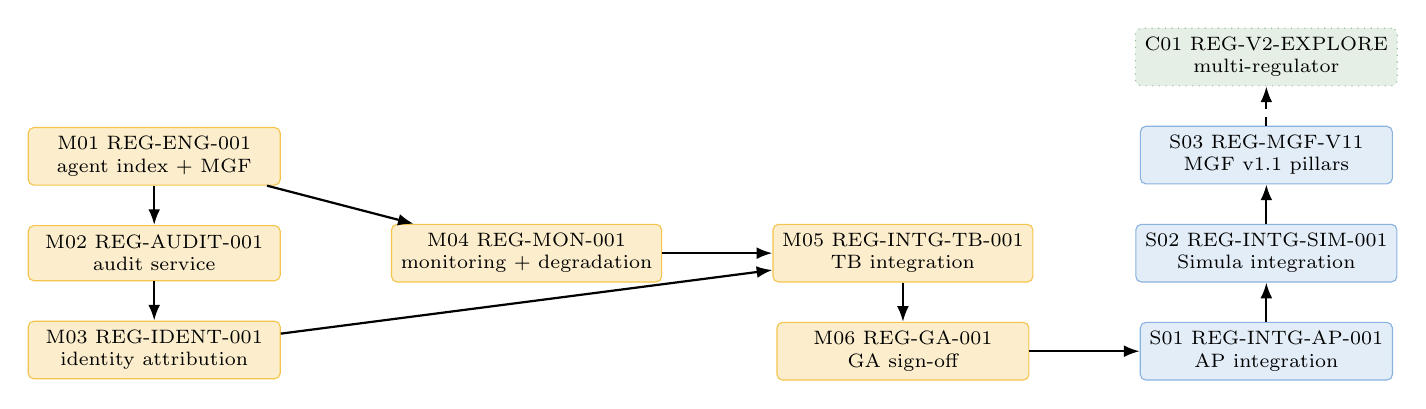
\begin{tikzpicture}[
node distance=5mm and 10mm,
must/.style={draw,rounded corners=2pt,align=center,font=\scriptsize,
fill=regamber!20,draw=regamber!70,
minimum height=7mm,minimum width=32mm},
should/.style={draw,rounded corners=2pt,align=center,font=\scriptsize,
fill=regblue!12,draw=regblue!50,
minimum height=7mm,minimum width=32mm},
could/.style={draw,rounded corners=2pt,align=center,font=\scriptsize,
fill=reggreen!12,draw=reggreen!50,dotted,
minimum height=7mm,minimum width=32mm},
dep/.style={-{Latex[length=2mm]},thick},
soft/.style={-{Latex[length=2mm]},thick,dashed}
]
\node[must] (m01) {M01 REG-ENG-001 \\ \scriptsize agent index + MGF};
\node[must,below=of m01] (m02) {M02 REG-AUDIT-001 \\ \scriptsize audit service};
\node[must,below=of m02] (m03) {M03 REG-IDENT-001 \\ \scriptsize identity attribution};
\node[must,right=14mm of m02] (m04) {M04 REG-MON-001 \\ \scriptsize monitoring + degradation};
\node[must,right=14mm of m04] (m05) {M05 REG-INTG-TB-001 \\ \scriptsize TB integration};
\node[must,below=of m05] (m06) {M06 REG-GA-001 \\ \scriptsize GA sign-off};
\node[should,right=14mm of m06] (s01) {S01 REG-INTG-AP-001 \\ \scriptsize AP integration};
\node[should,above=of s01] (s02) {S02 REG-INTG-SIM-001 \\ \scriptsize Simula integration};
\node[should,above=of s02] (s03) {S03 REG-MGF-V11 \\ \scriptsize MGF v1.1 pillars};
\node[could,above=of s03] (c01) {C01 REG-V2-EXPLORE \\ \scriptsize multi-regulator};

\draw[dep] (m01) -- (m02);
\draw[dep] (m01) -- (m04);
\draw[dep] (m02) -- (m03);
\draw[dep] (m03) -- (m05);
\draw[dep] (m04) -- (m05);
\draw[dep] (m05) -- (m06);
\draw[dep] (m06) -- (s01);
\draw[dep] (s01) -- (s02);
\draw[dep] (s02) -- (s03);
\draw[soft] (s03) -- (c01);
\end{tikzpicture}
\caption{Regulations dependency graph. Amber nodes are Must (critical
path); blue are Should (consumer-integration and MGF-pillar
allowance); dotted green are Could (discretionary). Solid arrows are
hard prerequisites; dashed arrows indicate conditional starts (the
target is unlocked when the upstream completes \emph{and} the v2.0
trigger in \cref{sec:reg-v2-trigger} fires).}
\label{fig:reg-dependency-graph}
\end{figure}

\section{Project milestones}\label{sec:reg-milestones}

\begin{table}[htbp]
\centering
\caption{Regulations v1.0 project milestones in dependency order.
Priority: M=Must (critical path), S=Should, C=Could, W=Won't.}
\label{tab:reg-milestones}
\footnotesize
\begin{tabularx}{\linewidth}{@{}l l l l X@{}}
\toprule
\textbf{ID} & \textbf{Prereq} & \textbf{Pri.} & \textbf{Ticket} & \textbf{Milestone} \\ \midrule
M01 & ---       & M & REG-ENG-001        & Agent index and MGF framework specification complete; conformance tooling passes the fixtures in \cref{ch:tooling}. \\
M02 & M01       & M & REG-AUDIT-001      & Audit service (reserve/complete, immutable storage) live in UAT; SEV1/SEV2 clean. \\
M03 & M02       & M & REG-IDENT-001      & Identity attribution wiring (\cref{ch:identity}) live in UAT; REG-MGF-2.1.2-002 compliance upgraded from \textit{missing} to \textit{partial}. \\
M04 & M01       & M & REG-MON-001        & Monitoring spec operational: circuit breaker plus graceful-degradation ladder (\cref{sec:degradation-ladder}). \\
M05 & M03, M04  & M & REG-INTG-TB-001    & First consumer (Trial Balance) integrated end-to-end; reserve/complete coverage $=$ 100\,\% on TB actions. \\
M06 & M05       & M & REG-GA-001         & GA sign-off (audit + identity + monitoring) on the TB integration. \\
M07 & M06       & M & REG-BC-REFRESH     & Business-case refresh and compliance attestation (first cycle after GA; then annual). \\
S01 & M06       & S & REG-INTG-AP-001    & Arabic AP integration: reserve/complete on AP actions; REG-MGF-2.1.2-002 becomes \textit{compliant} once AP live. \\
S02 & S01       & S & REG-INTG-SIM-001   & Simula integration: reserve/complete on Simula corpus-generation actions. \\
S03 & M06       & S & REG-MGF-V11        & MGF v1.1 pillar updates ingested and mapped to agent index. \\
C01 & S03 + \cref{sec:reg-v2-trigger} trigger & C & REG-V2-EXPLORE & v2.0 multi-regulator correlation scoped (beyond IMDA MGF). \\
C02 & M06       & C & REG-TUNE           & Quarterly conformance-tooling retraining from accept/edit telemetry. \\
W01 & ---       & W & REG-V1-REALTIME    & Real-time cross-project audit dashboards are \emph{not} in v1.0 scope. \\
W02 & ---       & W & REG-V1-MULTIREG    & Multi-regulator correlation is \emph{not} in v1.0 scope; single-regulator (IMDA MGF) only. \\
\bottomrule
\end{tabularx}
\end{table}

\noindent
The Must chain (M01 $\to$ M02 $\to$ M03/M04 $\to$ M05 $\to$ M06 $\to$
M07) is the critical path. The Should items (S01--S03) are the
primary \emph{schedule allowance}: additional consumer integrations
and MGF pillars can slip without affecting v1.0 sign-off. The Could
items are the \emph{scope allowance}: they may be cut to v1.1 without
renegotiation.

\section{Launch tiers and exit gates}\label{sec:reg-launch-tiers}

The project walks the four-tier ladder shared across SAP OSS Finance
projects. A tier is exited only when the named exit gate is satisfied;
slippage requires sponsor sign-off.

\begin{table}[htbp]
\centering
\caption{Regulations launch tiers. The exit gate defines the MoSCoW
items that must be closed to exit the tier.}
\label{tab:reg-launch-tiers}
\footnotesize
\begin{tabularx}{\linewidth}{@{}l l X@{}}
\toprule
\textbf{Tier} & \textbf{Scope} & \textbf{Exit gate (references MoSCoW IDs)} \\ \midrule
Alpha & Engineering only, DEV + UAT, conformance fixtures only. & M01, M02, M04 closed; conformance tooling green on fixtures; reproducibility of audit outputs confirmed on two consecutive runs. \\
Beta  & Audit + identity + monitoring live for one consumer project (TB) in UAT. & M03, M05 closed; parallel-run gate in the TB spec passes for one full cycle; no open SEV1/SEV2; audit coverage $=$ 100\,\% of in-scope TB actions. \\
GA (limited) & Audit + identity + monitoring live for TB in production. & M06 closed; Beta gate sustained for two consecutive cycles; kill-switch green; REG-MGF-2.1.2-002 at \textit{partial} (TB-only). \\
Full rollout & All three current consumer projects integrated (TB, AP, Simula). & S01 and S02 closed; REG-MGF-2.1.2-002 at \textit{compliant}; two quarterly reviews sustained; M07 complete; business-case refresh complete. \\
\bottomrule
\end{tabularx}
\end{table}

\section{Kill-switch conditions}\label{sec:reg-kill-switch}

The kill-switch is a pre-committed rulebook: a tripped condition enters
the action column without further debate. GFAIC and sponsor are
notified within 24 hours. The conditions are evaluated continuously
(on every cycle) and do not carry dates.

\begin{table}[htbp]
\centering
\caption{Regulations kill-switch.}
\label{tab:reg-kill-switch}
\footnotesize
\begin{tabularx}{\linewidth}{@{}l l X@{}}
\toprule
\textbf{Condition} & \textbf{Evaluation} & \textbf{Action} \\ \midrule
Audit-coverage gap (missed \texttt{reserve/complete} pair) detected in production & continuous & \textbf{Halt GA onboarding for all consumers}; incident-review before next integration. \\
Circuit breaker tripped with no successful graceful-degradation fallback for three consecutive cycles & per cycle & \textbf{Halt upstream LLM traffic}; fail over to cached/heuristic path; remediate before resuming. \\
Identity-attribution reconciliation fails (principal of record cannot be resolved) for $>$\,0.01\,\% of actions & per cycle & \textbf{Pause affected consumer}; block further reserves until remediated. \\
Any IMDA MGF finding attributable to the Regulations platform (audit, identity, monitoring) & continuous & \textbf{Halt rollout}; remediate before next wave. \\
Any consumer project declares red on a Regulations-supplied component & continuous & \textbf{Pause downstream Should}; re-plan at next steering. \\
\bottomrule
\end{tabularx}
\end{table}

\section{Shared-platform dependencies}\label{sec:reg-shared-deps}

This project depends on two shared-platform components (it supplies
the rest). Each is tracked here only as a dependency, not a commitment
this project can unilaterally adjust. Sequence is expressed in terms
of the Must item that first consumes the dependency, not in calendar
time.

\begin{table}[htbp]
\centering
\caption{Shared-platform dependencies.}
\label{tab:reg-shared-deps}
\footnotesize
\begin{tabularx}{\linewidth}{@{}l l l X@{}}
\toprule
\textbf{Component} & \textbf{Owner} & \textbf{First consumed by} & \textbf{Impact if late} \\ \midrule
Unified schema registry (\path{docs/schema/}) & Shared infra & M01 & Already \texttt{migration.status=complete}; no remaining risk. \\
vLLM hosting (\texttt{vllm-only} policy) & Shared platform & M04 & The graceful-degradation ladder (\cref{sec:degradation-ladder}) is the mitigation; this project is the \emph{owner} of that ladder for sibling consumers. \\
\bottomrule
\end{tabularx}
\end{table}

\noindent
Shared-platform dependencies are surfaced at monthly steering. If any
upstream owner declares \textbf{amber} or \textbf{red} on a component
in \cref{tab:reg-shared-deps}, the affected downstream Must milestone
is re-planned at the following steering.

\section{v2.0 expansion trigger}\label{sec:reg-v2-trigger}

The Could item C01 (REG-V2-EXPLORE) is unlocked only when all of the
following are observed after two consecutive quarters of full rollout
under v1.0:

\begin{itemize}
\item a second regulator framework (beyond IMDA MGF) is formally
adopted as in-scope by the AI Governance Working Group;
\item MGF v1.1 pillars (S03) are fully mapped and at \textit{compliant}
status;
\item business-case refresh (M07) explicitly budgets the v2.0
programme.
\end{itemize}

\noindent
If any of the three conditions fails, C01 remains in the Could column
and is re-evaluated at the next business-case refresh.

\section{Governance and business-case cadence}\label{sec:reg-governance}

\paragraph{Project governance.}
The Regulations project reports monthly to a project steering (AI
Governance Lead, Compliance Officer, Platform Engineer) and quarterly
to the cross-project GFAIC, which it also convenes. Monthly steering
accepts or rejects amber/red signals on Must items; GFAIC reviews
compliance posture and cross-project dependencies (this project's
consumer-integration Should items feed directly into sibling projects'
Must items).

\paragraph{Business-case refresh (M07).}
The business case that authorises this project is refreshed on the
following rhythm:

\begin{itemize}
\item \textbf{Mandatory refresh}: at the first cycle after GA, and
annually thereafter (ticket REG-BC-REFRESH, priority M in
\cref{tab:reg-milestones}). Refresh packet includes consumer
integration load assumptions, unit economics
and platform operating cost
realised vs.\ forecast, and a deviation statement against the
baseline.
\item \textbf{Trigger-based refresh}: any of
\begin{itemize}
\item consumer-project count in scope changes by $\ge\,1$
(new consumer adopts, or one is retired);
\item per-action audit cost changes by $\ge\,30$\,\%
(storage, indexing, identity-reconciliation throughput);
\item a new MGF pillar, a new regulator framework, or a
material change to REG-MGF-2.1.2-002;
\item any kill-switch in \cref{tab:reg-kill-switch} is
tripped.
\end{itemize}
\item \textbf{Owner}: AI Governance Lead. Approval routed through
the project steering and filed at
\path{docs/regulations/business-case/refresh-history.yaml}.
\end{itemize}
\chapter{Agent Implementation Instructions}\label{ch:agent-impl}

\section{Purpose and audience}
This chapter is the self-contained, intent-based instruction set for
implementing the \emph{Regulations} domain inside the unified SAP
OSS platform. Regulations plays two roles at once: it is a persona
surface (Compliance Officer) in its own right, \emph{and} it is the
horizontal runtime wrapper that governs the three other domains
(Arabic AP, TB, Simula) at every MCP call. This chapter is written
for LLM-driven and human implementation agents who will extend
existing services to realise both roles. It assumes only this PDF;
every platform decision, integration contract, and governance
obligation is restated here so that no companion document is
required. Existing chapters~\ref{ch:overview}--\ref{ch:reg-roadmap}
remain the normative source for the regulations domain itself; this
chapter tells future agents \emph{how} to build what those chapters
describe, \emph{where} to put it in the codebase, and \emph{how} it
plugs into the wider platform.

% !TEX root = ../master.tex
% =============================================================================
% MASTER PLATFORM CORE: Shared Intent-Based Instructions (Union)
% World-Class Version: HITL Gates, Process Integrity, and .clinerules Wiring
% =============================================================================

\section{Rules of Engagement for AI Agents}
\label{sec:agent-rules}

To ensure safety and architectural integrity, all implementation agents must adhere to the following Prime Directives:

\begin{enumerate}[label=\textsc{rule}-\arabic*:, leftmargin=2cm]
\item \textbf{Credential Protection.} Never log, print, or commit secrets. Use the \texttt{.secrets.example} pattern for all new integrations.
\item \textbf{Context Efficiency.} Prioritize surgical edits. Request only the minimum required file ranges to satisfy the task intent.
\item \textbf{Test-Driven Implementation.} No code is complete without a corresponding fixture in \texttt{tests/fixtures/} and a passing validation run.
\item \textbf{Self-Correction.} If a schema validation fails, the agent must diagnose the root cause (hallucination vs. schema drift) before re-attempting implementation.
\item \textbf{Safety Inheritance.} Domain-specific agent rules (\texttt{.clinerules}) may only \emph{tighten} (e.g., lower timeout, stricter precision), never \emph{loosen} regulatory constraints.
\end{enumerate}

\section{Agent Rule-Pack Architecture (.clinerules)}
\label{sec:agent-rule-packs}

The platform mandates a three-tier inheritance hierarchy for agent behavior. Implementation agents must load the relevant rule pack before starting any task.

\subsection{Inheritance Hierarchy}
\begin{enumerate}
\item \textbf{Repository-level (\texttt{/.clinerules}):} The baseline for all engineering and documentation standards.
\item \textbf{Intelligence-level (\texttt{/src/intelligence/.clinerules}):} The regulatory envelope (IMDA MGF) that wraps all domains.
\item \textbf{Domain-level (\texttt{/src/<domain>/.clinerules}):} Domain-specific constraints (e.g., Arabic character precision).
\end{enumerate}

\subsection{Safety-Critical Flags}
The following flags in the rule packs are subject to \textsc{rule-5} (Inherit, Never Weaken):
\begin{table}[htbp]
\centering
\footnotesize
\caption{Safety-Critical Agent Flags.}
\label{tab:safety-flags}
\begin{tabularx}{\textwidth}{@{}l X X@{}}
\toprule
\textbf{Flag} & \textbf{Parent Value (Regs)} & \textbf{Tightening Direction} \\
\midrule
\texttt{deny\_by\_default} & \texttt{true} & Invariant (Cannot be set to false). \\
\texttt{require\_identity} & \texttt{true} & Invariant (Cannot be bypassed). \\
\texttt{max\_retries} & \texttt{3} & May only \emph{decrease}. \\
\texttt{timeout\_ms} & \texttt{30000} & May only \emph{decrease}. \\
\bottomrule
\end{tabularx}
\end{table}

\section{Platform Overview --- One Codebase, One Instance}
\label{sec:agent-platform-overview}

\subsection{Integration Stance}
The SAP OSS platform is delivered as a single codebase that runs as a single logical instance. All cross-cutting concerns are hosted by existing services.

\begin{adrbox}{{One Codebase, One Instance}}
To minimize integration latency and eliminate distributed-system failure modes (e.g., partial partitions), we mandate a single logical instance. All cross-domain orchestration happens via the MCP Gateway layer.
\end{adrbox}

\subsection{Platform Integration Map}
\label{sec:platform-map}

\begin{figure}[htbp]
\centering
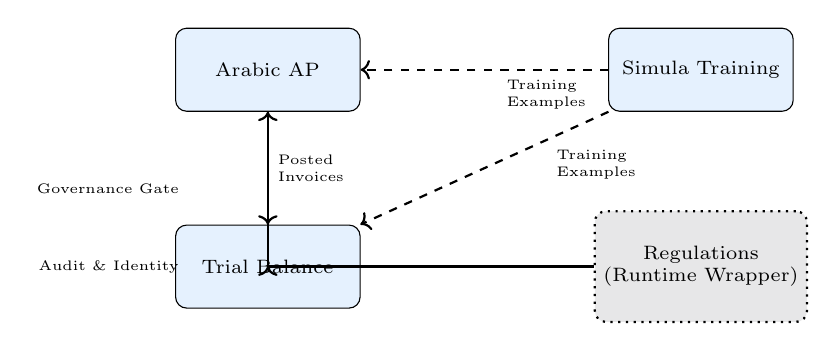
\begin{tikzpicture}[
node distance=2.5cm,
auto,
block/.style={rectangle, draw, rounded corners, fill=sapblue!10, text width=6em, text centered, minimum height=3em, font=\scriptsize},
regs/.style={rectangle, draw, rounded corners, fill=sapgrey!20, text width=7em, text centered, minimum height=4em, thick, dotted, font=\scriptsize}
]
\node (arabic) [block] {Arabic AP};
\node (tb) [block, below of=arabic] {Trial Balance};
\node (simula) [block, right of=arabic, node distance=5.5cm] {Simula Training};
\node (regs) [regs, below of=simula] {Regulations (Runtime Wrapper)};

\draw [->, thick] (arabic) -- node [align=left, font=\tiny] {Posted\\Invoices} (tb);
\draw [->, thick, dashed] (simula) -- node [align=left, font=\tiny, near start] {Training\\Examples} (arabic);
\draw [->, thick, dashed] (simula) -- node [align=left, font=\tiny, near start] {Training\\Examples} (tb);
\draw [->, thick] (regs) -| node [font=\tiny, near end, xshift=-1cm] {Governance Gate} (arabic);
\draw [->, thick] (regs) -| node [font=\tiny, near end, xshift=-1cm] {Audit \& Identity} (tb);
\end{tikzpicture}
\caption{Cross-domain interaction and unified data flow map. Detailed governance logic is defined in \cref{reg:ch:mgf}.}
\end{figure}

\section{Transactional Sequence Diagrams}
\label{sec:agent-sequences}

Implementation agents must adhere to the temporal logic defined below. Every cross-domain request MUST be brokered by the Regulations Wrapper.

\subsection{Universal Governance Handshake}
This sequence applies to \textbf{all} platform service calls.

\begin{figure}[htbp]
\centering
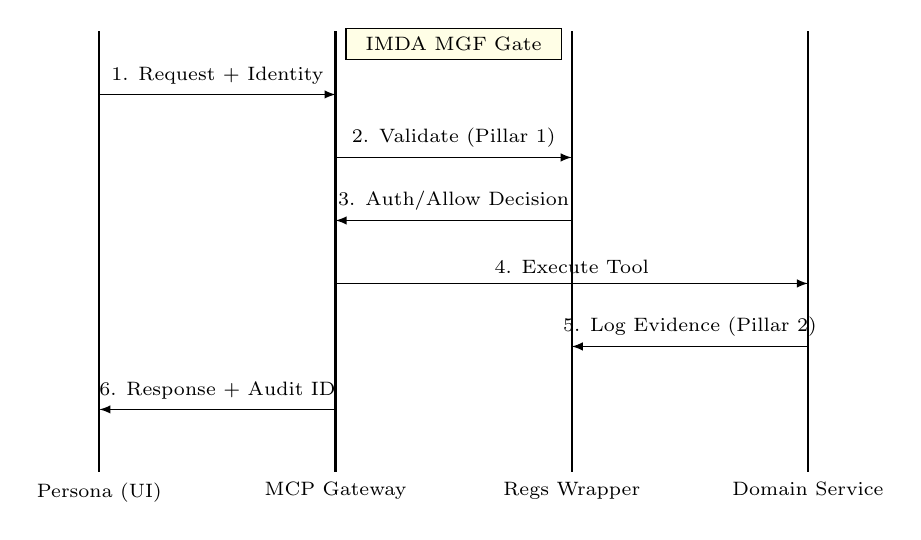
\begin{tikzpicture}[x=1cm, y=-0.8cm, font=\scriptsize]
% Lifelines
\draw[thick] (0,0) -- (0,7) node[below] {Persona (UI)};
\draw[thick] (3,0) -- (3,7) node[below] {MCP Gateway};
\draw[thick] (6,0) -- (6,7) node[below] {Regs Wrapper};
\draw[thick] (9,0) -- (9,7) node[below] {Domain Service};

% Interaction
\draw[->, >=latex] (0,1) -- node[above] {1. Request + Identity} (3,1);
\draw[->, >=latex] (3,2) -- node[above] {2. Validate (Pillar 1)} (6,2);
\draw[<-, >=latex] (3,3) -- node[above] {3. Auth/Allow Decision} (6,3);
\draw[->, >=latex] (3,4) -- node[above] {4. Execute Tool} (9,4);
\draw[->, >=latex] (9,5) -- node[above] {5. Log Evidence (Pillar 2)} (6,5);
\draw[<-, >=latex] (0,6) -- node[above] {6. Response + Audit ID} (3,6);

\node[draw, fill=yellow!10, text width=2.5cm, align=center] at (4.5,0.2) {IMDA MGF Gate};
\end{tikzpicture}
\caption{Standard platform handshake for governed tool execution. Audit schemas are detailed in \cref{reg:ch:identity}.}
\end{figure}

\subsection{Arabic AP Golden Path}
Temporal flow for invoice processing with Arabic context.

\begin{figure}[htbp]
\centering
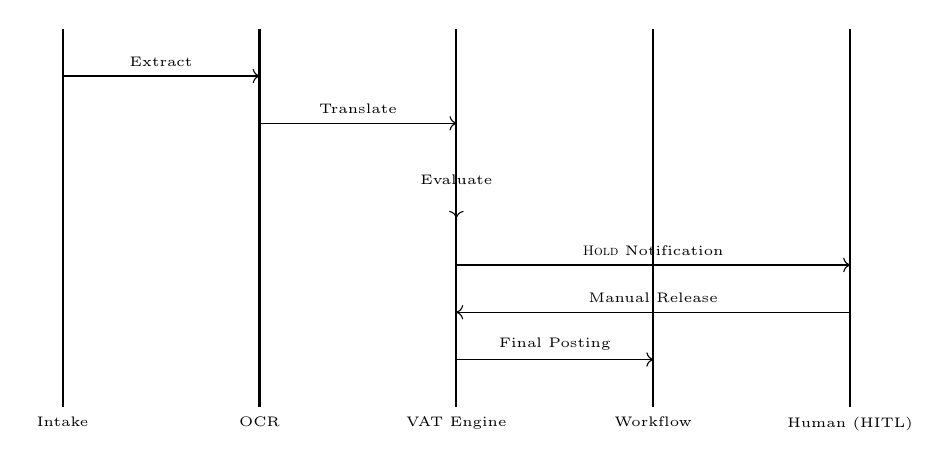
\begin{tikzpicture}[x=1cm, y=-0.6cm, font=\tiny]
\draw[thick] (0,0) -- (0,8) node[below] {Intake};
\draw[thick] (2.5,0) -- (2.5,8) node[below] {OCR};
\draw[thick] (5,0) -- (5,8) node[below] {VAT Engine};
\draw[thick] (7.5,0) -- (7.5,8) node[below] {Workflow};
\draw[thick] (10,0) -- (10,8) node[below] {Human (HITL)};

\draw[->] (0,1) -- node[above] {Extract} (2.5,1);
\draw[->] (2.5,2) -- node[above] {Translate} (5,2);
\draw[->] (5,3) -- node[above] {Evaluate} (5,4); % Internal loop
\draw[->] (5,5) -- node[above] {\textsc{Hold} Notification} (10,5);
\draw[<-] (5,6) -- node[above] {Manual Release} (10,6);
\draw[->] (5,7) -- node[above] {Final Posting} (7.5,7);
\end{tikzpicture}
\caption{Arabic AP sequence: Scanned PDF to Release. VAT rules are specified in \cref{ar:ch:vat}.}
\end{figure}

\section{Compute and Resource Alignment}
\label{sec:hardware-profiles}

AI algorithms are calibrated for the reference infrastructure established in the domain chapters:

\begin{table}[htbp]
\centering
\footnotesize
\caption{Infrastructure Reference Profiles.}
\label{tab:hardware-profiles}
\begin{tabularx}{\textwidth}{@{}l X X@{}}
\toprule
\textbf{Workload} & \textbf{Reference Hardware} & \textbf{Performance Target} \\
\midrule
LLM Inference & NVIDIA L40S (48GB) & AWQ 4-bit / p95 < 2s \\
Embeddings & NVIDIA A100 (40/80GB) & FP16 / p99 < 500ms \\
Simula Training & NVIDIA A100 SXM4 cluster & BF16 throughput parity \\
\bottomrule
\end{tabularx}
\end{table}

\section{Human-in-the-Loop (HITL) Critical Gates}
\label{sec:hitl-gates}

The following "Four-Eyes" gates are mandatory. AI agents must implement the "Awaiting Sign-off" state for these actions:
\begin{itemize}
\item \textbf{VAT Release:} No invoice marked as \textsc{hold} can be released without human review (see \cref{ar:ch:ap}).
\item \textbf{Anomaly Override:} Statistical outliers ($3\sigma$) cannot be dismissed by AI; only "Confirmed" or "Triaged" by human (see \cref{tb:ch:controls}).
\item \textbf{Journal Posting:} Agents may \emph{draft} journal entries, but only the Financial Controller persona can \emph{commit} to S/4HANA (see \cref{tb:ch:controls-engine}).
\end{itemize}

\section{Registry Integrity \& Live Status}
\label{sec:registry-integrity}

Before initiating any schema-dependent task, implementation agents must verify the live status of the Unified Schema Registry (see \cref{sim:chap:schema}).
\begin{adrbox}{Registry First}
If \texttt{docs/schema/registry.json} is out of sync with the codebase, the agent must halt and emit a \textsc{schema-mismatch} event.
\end{adrbox}

\section{Master Implementation Manifest (Union)}
Implementation runs in three waves across the entire platform.

\subsection*{Wave 1 --- Foundations}
\begin{itemize}
\item \textbf{Simula:} Implement HANA schema extraction pipeline (MCP discovery). See \cref{sim:chap:extraction}.
\item \textbf{Regulations:} Implement IMDA MGF Pillar 1 logic (Tool allow-list). See \cref{reg:ch:mgf}.
\item \textbf{Arabic:} Implement Invoice Intake \& OCR Gateway. See \cref{ar:ch:ai}.
\item \textbf{Trial Balance:} Implement identity-attribution wiring. See \cref{reg:ch:identity}.
\end{itemize}

\subsection*{Wave 2 --- Core Domain Build-out}
\begin{itemize}
\item \textbf{Trial Balance:} Implement Controls \& Commentary Engine (3$\sigma$ anomaly logic). See \cref{tb:ch:ai,tb:ch:controls-engine}.
\item \textbf{Arabic:} Implement multi-country VAT Engine (Saudi, UAE, Bahrain, Oman). See \cref{ar:ch:vat,ar:ch:vat-impl}.
\item \textbf{Simula:} Implement Taxonomy Generation \& Agentic Data Synthesis. See \cref{sim:chap:taxonomy,sim:chap:generator}.
\item \textbf{Trial Balance:} Realise 28-state BPMN workflow (\texttt{tb-review-glo}). See \cref{tb:ch:workflow}.
\end{itemize}

\subsection*{Wave 3 --- Hardening}
\begin{itemize}
\item \textbf{Regulations:} Implement Per-Request Identity Attribution. See \cref{reg:ch:identity}.
\item \textbf{Trial Balance:} Deliver Human Review Dashboard. See \cref{tb:ch:review-dashboard}.
\item \textbf{Simula:} Deliver test fixtures and testing at 85\% coverage. See \cref{sim:ch:test-fixtures,sim:ch:testing}.
\item \textbf{Regulations:} Wire Emergent-Capability monitoring. See \cref{reg:ch:monitoring}.
\end{itemize}

\section{Governance Obligations (IMDA MGF)}
The regulations domain wraps all service calls at runtime. Agents must implement the following hooks in every domain:
\begin{itemize}
\item \textbf{Pillar 1:} Tool allow-list enforcement (deny-by-default).
\item \textbf{Pillar 2:} Traceability via the identity attribution envelope.
\item \textbf{Pillar 3:} Metric emission to the monitoring sink.
\end{itemize}
Detailed pillar requirements are defined in \cref{reg:ch:mgf}.

\section{FMEA: Failure Mode and Effects Analysis for AI}
\label{sec:fmea-ai}

The following analysis identifies critical AI failure modes within the Regulations governance runtime and their deterministic mitigations.

\begin{table}[htbp]
\centering
\footnotesize
\caption{FMEA for Regulations AI Governance Pipeline.}
\label{tab:reg-fmea}
\begin{tabularx}{\textwidth}{@{}l X X X@{}}
\toprule
\textbf{Failure Mode} & \textbf{Symptom} & \textbf{Impact} & \textbf{Technical Mitigation} \\
\midrule
Entitlement Drift & Persona allowed to call a non-allow-listed MCP tool. & Critical (Security) & Deny-by-default hard gate in MCP Gateway middleware. \\
Audit Omission & High-risk action emitted without Identity Envelope. & High (Compliance) & Mandatory envelope-check hook in PAL evidence-writer. \\
Monitoring Blindspot & Emergent capability detected but metrics not emitted. & Medium (Risk) & Periodic 'Heartbeat' probe to Monitoring Sink. \\
\bottomrule
\end{tabularx}
\end{table}

\section{This domain in context}
\label{sec:agent-domain-context}
Regulations is unique among the four domains: it is both a persona
surface (Compliance Officer) and the horizontal runtime wrapper that
governs Arabic, TB, and Simula at every MCP call. As a persona
surface, its working view is the governance dashboard surfaced
through the shared workspace shell and gated by regulations
entitlements. As a runtime wrapper, it has no separate service of
its own: the governance hooks are attached to the gateway and to
ai-core-pal, and they are exercised on every call the platform
handles. Its entry points are (a)~any inbound MCP call into any
domain, which must pass through the governance gate, and (b)~the
Compliance Officer's review queue. Its exit points are
(a)~governance decisions (allow, deny, degrade) returned to the
gateway, (b)~evidence records written to the shared governance
store, and (c)~conformance reports for auditors.

\section{Schema contribution}
\label{sec:agent-schema-contrib}
Regulations owns the schemas catalogued in chapter~\ref{ch:schema}
and listed in~\ref{tab:schemas}. The canonical set is the
requirement record (the linkage schema between source rule, artefact,
and evidence), the conformance-tool record, the enum vocabularies
in~\ref{tab:enums}, the capability-monitoring metrics record
(chapter~\ref{ch:monitoring}), and the identity and audit-event
schemas in chapter~\ref{ch:identity}. These schemas live under
\texttt{docs/latex/specs/regulations/} as normative text and under
\texttt{structured/schema/} as the JSON Schema artefacts consumed at
runtime. Registration in the unified registry is additive: each
schema is listed in
\texttt{src/intelligence/ai-core-pal/data\_products/registry.yaml}
with its URI, owning domain (\texttt{regulations}), security class
(\texttt{confidential}), and LLM routing (\texttt{vllm-only}),
following the ODPS~4.1 pattern. Simula consumes these schemas
directly as inputs to its extraction pipeline; it does not transform
them. Regulations' \texttt{requirement.schema.json} is a distinct
URI from TB's \texttt{requirement.schema.json}; the two files are
not merged.

\section{Persona and MCP allow-list}
\label{sec:agent-persona}
\begin{itemize}
\item \textbf{Persona id:} \texttt{compliance-officer}.
\item \textbf{Roles:} requirement registration, governance-policy
authoring, conformance-run triage, emergent-capability review,
audit-trail inspection.
\item \textbf{Entitlements:} read/write on the requirement record,
conformance-tool record, capability-monitoring record, and the
identity-and-audit schemas; read on every other domain's
evidence output (needed to assemble conformance reports);
override-write on governance-decision records (rare, audit-logged).
\item \textbf{UI route:} \texttt{/governance/\{tenant\}/dashboard}
on the shared workspace shell; surfaced only to callers whose
entitlement set includes \texttt{compliance-officer}.
\item \textbf{MCP tool allow-list:}
\texttt{gov.requirement.register}, \texttt{gov.policy.publish},
\texttt{gov.conformance.run}, \texttt{gov.conformance.report},
\texttt{gov.monitor.query}, \texttt{gov.audit.query},
\texttt{gov.identity.attest}. All other MCP tools are denied by
default per IMDA MGF pillar~1.
\end{itemize}

\section{Agent Rule-Pack Binding}
\label{sec:agent-rule-binding}
Before initiating any task in this domain, the agent MUST load the following rule packs in order:
\begin{enumerate}
\item \filepath{.clinerules} (Global Standards)
\item \filepath{src/intelligence/.clinerules} (Regulations Envelope)
\end{enumerate}

\section{Implementation tasks for this domain}
\label{sec:agent-tasks}
The tasks below are intent-based: each task states the outcome a
future agent must achieve and the location in the existing codebase
where the work belongs. None of them contains code; each task binds
to the regulations chapters that define the required behaviour.

\subsection*{Task R1 --- MGF four-pillar runtime checks}
\textbf{Intent.} Realise the four IMDA MGF pillars defined in
chapter~\ref{ch:mgf} as runtime checks that run on every inbound MCP
call in every non-regulations domain.

\begin{adrbox}{Why Pillars over Flat Rules?}
We adopted the IMDA MGF Pillar structure to ensure that governance is not just a 'checklist' but a runtime operational model that scales as new domains (e.g., ESG, Supply Chain) are onboarded.
\end{adrbox}

\textbf{In-scope.} Pillar~1 (assess and bound) via allow-list
enforcement at the gateway; pillars~2--4 via the evidence and
disclosure hooks on ai-core-pal; pillar binding per
\S\ref{sec:mgf-p1} and~\ref{tab:p1}.
\textbf{Out-of-scope.} Re-implementing the MGF rule source; the
source document is frozen and referenced by its sha in~\ref{tab:src-hashes}.
\textbf{Paths to extend.} Governance hooks in the gateway; evidence
writer in ai-core-pal.
\textbf{Definition of done.} Every allow/deny decision references a
pillar; denials are surfaced to the caller with a stable error code;
evidence records for each pillar are written for every call.

\textbf{Autonomous Verification (Agent Logic):}
\begin{lstlisting}[language=jsonx]
// Verify Task R1
{
"test_fixture": "tests/fixtures/regulations/unauthorized_call.json",
"expected_outcome": "http_status == 403",
"validation_command": "make test-gov-runtime --pillar=1"
}
\end{lstlisting}

\textbf{Verification.} Running any non-regulations domain's golden
sample produces a governance evidence record per pillar per call;
\texttt{make spec-regulations} remains green.

\subsection*{Task R2 --- AI Agent Index mapping}
\textbf{Intent.} Operationalise the 2025 AI Agent Index
transparency requirements listed in chapter~\ref{ch:agent-index},
especially~\ref{tab:agentidx-reqs}.
\textbf{In-scope.} Requirement registration per row; verification
runners that check that each agent surface exposes the required
transparency metadata (model, training set summary, known failure
modes).
\textbf{Out-of-scope.} Public disclosure portals.
\textbf{Paths to extend.} Requirement record loader; governance
dashboard transparency tab.
\textbf{Definition of done.} Every row in~\ref{tab:agentidx-reqs}
maps to a runnable verification; failures show up on the dashboard.
\textbf{Verification.} Conformance runner report 100\% of Agent
Index requirements either passing or explicitly waived with
attached evidence.

\subsection*{Task R3 --- Empirical evaluation hookup}
\textbf{Intent.} Encode the requirements extracted from Ju \& Aral
(2026) in chapter~\ref{ch:empirical} and~\ref{tab:jural-reqs} as
runnable empirical checks against the platform.
\textbf{In-scope.} Test harness that executes the Ju \& Aral
requirements on Arabic, TB, and Simula outputs; periodic run
cadence.
\textbf{Out-of-scope.} Adding new empirical studies.
\textbf{Paths to extend.} Regulations test harness colocated with
chapter~\ref{ch:testing} fixtures; scheduler hook.
\textbf{Definition of done.} Every requirement
in~\ref{tab:jural-reqs} has a callable check; the harness reports
pass/fail per requirement on the most recent platform build.
\textbf{Verification.} Harness run produces a per-requirement
report; failures block the CI gate.

\subsection*{Task R4 --- Conformance tooling integration}
\textbf{Intent.} Integrate AI Verify 2.0 and Moonshot CI/CD 1.1.0
per chapter~\ref{ch:tooling} and the coverage map
in~\ref{fig:tool-coverage}.
\textbf{In-scope.} AI Verify plug-ins listed in~\ref{tab:av-plugins}
and Moonshot benchmarks listed in~\ref{tab:ms-benchmarks};
conformance-run CLI exposed to the Compliance Officer persona.
\textbf{Out-of-scope.} Upstream changes to AI Verify or Moonshot.
\textbf{Paths to extend.} Conformance harness invoked from the
gateway; dashboard run-history view.
\textbf{Definition of done.} Running the conformance suite against
the platform produces a unified report covering every plug-in and
every benchmark in the two tables.
\textbf{Verification.} \texttt{gov.conformance.run} returns a report
that validates against the conformance-tool schema.

\subsection*{Task R5 --- Capability monitoring}
\textbf{Intent.} Deliver the capability monitoring specification in
chapter~\ref{ch:monitoring}, with the architecture
in~\ref{fig:monitor-arch} and the metrics in~\ref{tab:monitor-metrics}.
\textbf{In-scope.} Metrics collection at each of the collection
points; storage in the monitoring sink; threshold-based alerts.
\textbf{Out-of-scope.} Long-term analytics warehouse.
\textbf{Paths to extend.} Monitoring hooks on ai-core-pal; alert
router.
\textbf{Definition of done.} Every metric in~\ref{tab:monitor-metrics}
is emitted in production; alerts fire on the thresholds the chapter
defines.
\textbf{Verification.} Synthetic load test shows every required
metric at the sink; alerting simulator triggers every configured
alert.

\subsection*{Task R6 --- Identity attribution}
\textbf{Intent.} Realise per-request identity attribution per
chapter~\ref{ch:identity}, including the agent identity, request
identity, and audit-event schemas.
\textbf{In-scope.} Identity envelope construction at the gateway;
propagation through every domain service call; audit writer that
emits every required event.
\textbf{Out-of-scope.} Replacing the existing authentication
backend.
\textbf{Paths to extend.} Gateway identity middleware; audit writer
in ai-core-pal.
\textbf{Definition of done.} No MCP call leaves the gateway without
a complete identity envelope; every required audit event is written
with the schema's required fields.
\textbf{Verification.} Audit query over a test run surfaces every
event class; absent or partial envelopes fail the CI gate.

\subsection*{Task R7 --- Testing}
\textbf{Intent.} Deliver the regulations testing specification in
chapter~\ref{ch:testing} at the coverage thresholds
in~\ref{tab:reg-coverage}.
\textbf{In-scope.} Regulation fixtures, conformance-tool fixtures,
unit tests for requirement parsing, integration tests over the
governance gate.
\textbf{Out-of-scope.} Load benchmarking beyond what
chapter~\ref{ch:testing} defines.
\textbf{Paths to extend.} Test directory colocated with the
regulations service code.
\textbf{Definition of done.} Coverage meets~\ref{tab:reg-coverage};
CI gates block regressions.
\textbf{Verification.} \texttt{make spec-regulations} remains green;
the regulations test entry points all run.


\section{Governance obligations applied to this domain}
\label{sec:agent-governance}
Regulations is both the persona surface and the wrapper. The four
obligations therefore apply to regulations in two ways: as the
author of the obligations (canonical source in this spec's chapters)
and as a subject of the obligations (like every other domain, its
own MCP calls pass through the governance gate).

\begin{itemize}
\item \textbf{IMDA MGF four pillars} (chapter~\ref{ch:mgf}). The
regulations service authors the pillar definitions; it also
executes them against its own MCP tools. Pillar~1 enforcement
applies the allow-list in \S\ref{sec:agent-persona},
deny-by-default.
\item \textbf{Identity attribution} (chapter~\ref{ch:identity}).
Regulations owns the identity and audit-event schemas; its own
MCP calls carry the identity envelope like any other domain.
\item \textbf{Emergent-capability monitoring}
(chapter~\ref{ch:monitoring}). Regulations authors the metrics
model; governance decisions, conformance runs, and audit queries
are themselves instrumented.
\item \textbf{Conformance tooling} (chapter~\ref{ch:tooling}).
Regulations integrates AI Verify 2.0 and Moonshot CI/CD 1.1.0
as runnable suites; the regulations service's own behaviour is
included in every conformance run.
\end{itemize}

\section{Cross-spec integration --- full detail}
\label{sec:agent-integration}

\subsection{With Arabic AP}
Regulations wraps Arabic at runtime. Every Arabic MCP call is
brokered through the regulations governance gate, which applies
pillars~1--4 of IMDA MGF, attaches the identity envelope, and routes
emergent-capability metrics to the monitoring store. Arabic exports
the invoice record, VAT compliance checklist, and payment
instruction schemas under \texttt{structured/schema/} and registers
its MCP tools with the gateway; the governance gate consumes those
registrations but adds no Arabic-specific code paths. Conformance
tests defined here execute against the Arabic service as part of
the platform CI gate.

\subsection{With Trial Balance}
Regulations wraps TB at runtime. Every TB MCP call is brokered
through the regulations governance gate, which applies pillars~1--4
of IMDA MGF, attaches the identity envelope, and routes
emergent-capability metrics to the monitoring store. TB exports the
control record, decision-point record, workflow record, and its own
\texttt{requirement.schema.json} under \texttt{structured/schema/}.
Regulations' \texttt{requirement.schema.json} is a distinct URI
from TB's; no schema merge takes place.

\subsection{With Regulations}
Regulations exports the requirement record, conformance-tool record,
enum vocabularies, capability-monitoring metrics record, and the
identity and audit-event schemas under \texttt{structured/schema/};
registers the MCP tools enumerated in \S\ref{sec:agent-persona};
and applies the four governance hooks in
\S\ref{sec:agent-governance} to every call it serves --- including
its own. External consumers (Arabic, TB, Simula) see regulations
only through these contracts and through the wrapper; there are no
private back-channels.

\subsection{With Simula}
Regulations wraps Simula at runtime in the same way it wraps Arabic
and TB. Simula also consumes regulations' schemas (requirement,
conformance-tool, monitoring metrics, identity and audit) as
training input. The contract is schema-in,
\texttt{TrainingExample}-out: Simula reads the regulations schema
set; it produces \texttt{TrainingExample} records. Simula does not
call regulations MCP tools at runtime and does not share state with
the governance dashboard. No cross-domain operational envelope is
introduced.

\section{Wave assignment and sequencing}
\label{sec:agent-waves}
Implementation runs in three waves.

\begin{itemize}
\item \textbf{Wave 1 --- foundations.} Identity schema
(chapter~\ref{ch:identity}) frozen; gateway identity envelope;
persona-gated surface for the Compliance Officer; unified schema
registry entries for regulations schemas.
\item \textbf{Wave 2 --- governance runtime.} Tasks R1, R4, R5, R6
above. Prerequisites: Wave~1 complete; Simula Wave~1 extraction
pipeline available for monitoring metrics ingestion.
\item \textbf{Wave 3 --- evaluation and hardening.} Tasks R2, R3,
R7. Prerequisites: Wave~2 complete; monitoring sink live; all
non-regulations domains exposing their conformance entry
points.
\end{itemize}

Regulations is the critical-path domain for Wave~1 (identity) and
Wave~2 (governance runtime). Other domains block on regulations'
Wave~1 completion.

\section{Acceptance criteria (platform-wide)}
\label{sec:agent-acceptance}
When all four chapter~12 instruction sets are implemented, the
platform satisfies the following invariants:

\begin{enumerate}
\item \textbf{One instance.} A single codebase runs a single
logical instance; no domain ships as a separate product.
\item \textbf{Persona-gated surfaces.} The four personas each
reach a tailored UI on the shared shell; no route, MCP tool, or
data product is visible outside its persona's entitlement set.
\item \textbf{Unified registry.} Every schema in use is listed in
the ODPS~4.1 registry under its owning domain; validators
resolve \texttt{\$ref}s through the unified registry only.
\item \textbf{No schema merges.} The two
\texttt{requirement.schema.json} files in TB and regulations
remain distinct; no cross-domain composite schemas are produced.
\item \textbf{No cross-domain operational envelope.} Runtime
orchestration stays within each domain's service; only Simula
consumes other domains' outputs, and only as training input.
\item \textbf{Governance wraps all three non-regulations domains.}
Arabic, TB, and Simula service calls pass through the
regulations runtime wrapper without exception.
\end{enumerate}

\section{References}
\label{sec:agent-references}
Within-spec references:
chapter~\ref{ch:overview} (overview),
chapter~\ref{ch:schema} (data schema),
chapter~\ref{ch:mgf} (IMDA MGF framework),
chapter~\ref{ch:agent-index} (AI Agent Index),
chapter~\ref{ch:empirical} (Ju \& Aral empirical evidence),
chapter~\ref{ch:tooling} (conformance tooling),
chapter~\ref{ch:refs} (references and traceability),
chapter~\ref{ch:monitoring} (capability monitoring),
chapter~\ref{ch:testing} (testing specification),
chapter~\ref{ch:identity} (identity attribution),
chapter~\ref{ch:reg-roadmap} (project roadmap).

Peer chapter~12 instruction sets for the other three domains (each
is self-contained; consult directly when operating in that domain):
\begin{itemize}
\item Arabic AP:
\texttt{docs/latex/specs/arabic/chapters/12-implementation-instructions.tex}.
\item Trial Balance:
\texttt{docs/latex/specs/tb/chapters/12-implementation-instructions.tex}.
\item Simula:
\texttt{docs/latex/specs/simula/chapters/12-implementation-instructions.tex}.
\end{itemize}

Shared platform artefacts:
\begin{itemize}
\item ODPS~4.1 registry:
\texttt{src/intelligence/ai-core-pal/data\_products/registry.yaml}.
\item Schema pipeline and resolver:
\texttt{src/intelligence/schema\_pipeline/}.
\item Training pipeline (Simula):
\texttt{src/training/pipeline/}.
\item Shared workspace shell:
\texttt{generativeUI/training-webcomponents-ngx}.
\end{itemize}

% --- Incorporated Universal Chapters ---
\chapter{Global Wave-Dependency Manifest}
\label{ch:global-dependencies}

\section{Critical Path Visualization (Waves 1--3)}
The following chart defines the normative sequencing for implementation agents. A task in a later wave cannot be marked \textsc{complete} until its prerequisites in an earlier wave are validated.

\begin{figure}[htbp]
\centering
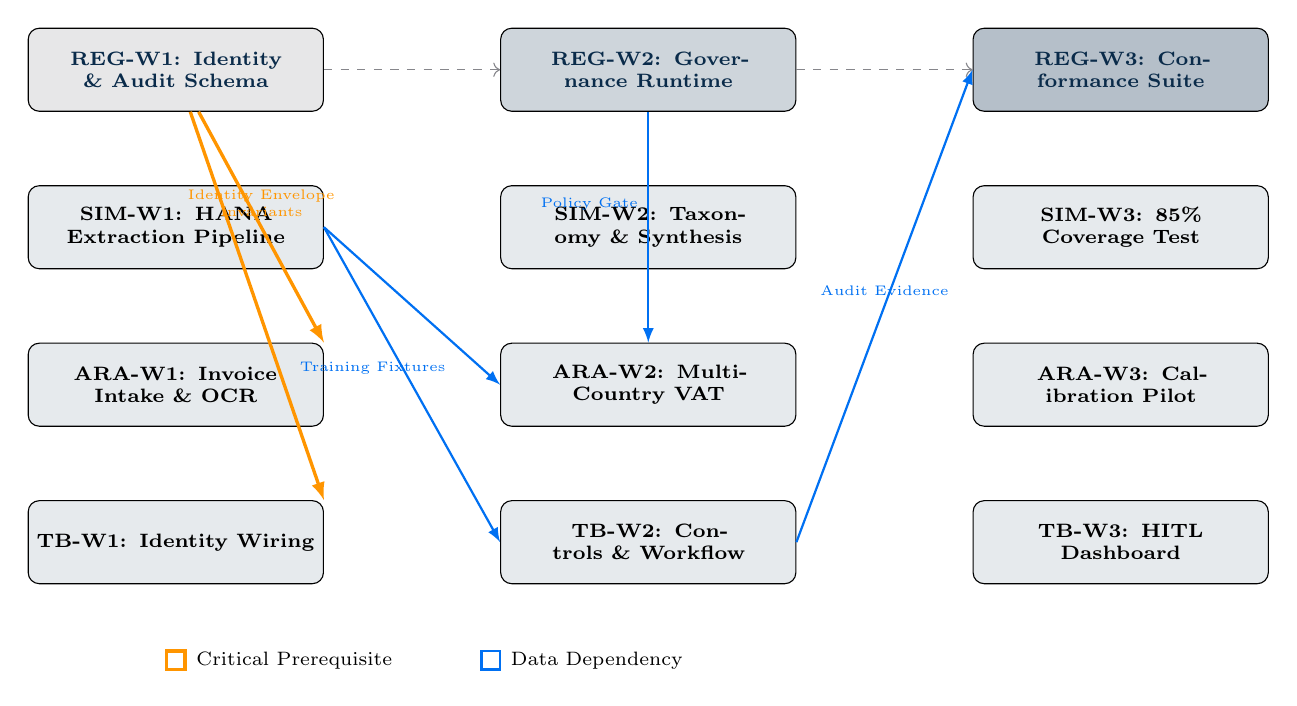
\begin{tikzpicture}[
node distance=1.5cm,
auto,
wavebox/.style={rectangle, draw, rounded corners, fill=sapmidnight!10, text width=10em, text centered, minimum height=3em, font=\scriptsize\bfseries},
dep/.style={->, >=latex, thick, sapblue},
critical/.style={->, >=latex, very thick, sapamber}
]
% --- Wave 1: Foundations ---
\node (r1) [wavebox, fill=sapgrey!20] {\textcolor{sapmidnight}{REG-W1: Identity \& Audit Schema}};
\node (s1) [wavebox, below of=r1, yshift=-0.5cm] {SIM-W1: HANA Extraction Pipeline};
\node (a1) [wavebox, below of=s1, yshift=-0.5cm] {ARA-W1: Invoice Intake \& OCR};
\node (t1) [wavebox, below of=a1, yshift=-0.5cm] {TB-W1: Identity Wiring};

% --- Wave 2: Core Build-out ---
\node (r2) [wavebox, right of=r1, xshift=4.5cm, fill=sapmidnight!20] {\textcolor{sapmidnight}{REG-W2: Governance Runtime}};
\node (s2) [wavebox, right of=s1, xshift=4.5cm] {SIM-W2: Taxonomy \& Synthesis};
\node (a2) [wavebox, right of=a1, xshift=4.5cm] {ARA-W2: Multi-Country VAT};
\node (t2) [wavebox, right of=t1, xshift=4.5cm] {TB-W2: Controls \& Workflow};

% --- Wave 3: Hardening ---
\node (r3) [wavebox, right of=r2, xshift=4.5cm, fill=sapmidnight!30] {\textcolor{sapmidnight}{REG-W3: Conformance Suite}};
\node (s3) [wavebox, right of=s2, xshift=4.5cm] {SIM-W3: 85\% Coverage Test};
\node (a3) [wavebox, right of=a2, xshift=4.5cm] {ARA-W3: Calibration Pilot};
\node (t3) [wavebox, right of=t2, xshift=4.5cm] {TB-W3: HITL Dashboard};

% --- Cross-Domain Dependencies (The Critical Path) ---
\draw [critical] (r1) -- node [above, font=\tiny, align=center] {Identity Envelope\\Invariants} (a1.north east);
\draw [critical] (r1) -- (t1.north east);
\draw [dep] (s1.east) -- node [above, font=\tiny, xshift=-0.5cm] {Training Fixtures} (t2.west);
\draw [dep] (s1.east) -- (a2.west);
\draw [dep] (r2.south) -- node [left, font=\tiny, yshift=0.3cm] {Policy Gate} (a2.north);
\draw [dep] (t2.east) -- node [above, font=\tiny] {Audit Evidence} (r3.west);

% --- Wave Transitions ---
\draw [->, dashed, sapgrey] (r1.east) -- (r2.west);
\draw [->, dashed, sapgrey] (r2.east) -- (r3.west);

% --- Legend ---
\node[draw, sapamber, very thick, label=right:\scriptsize Critical Prerequisite] at (0,-7.5) {};
\node[draw, sapblue, thick, label=right:\scriptsize Data Dependency, xshift=4cm] at (0,-7.5) {};

\end{tikzpicture}
\caption{Cross-specification dependency graph: The blueprint for platform rollout.}
\end{figure}

\section{Inter-Domain Prerequisite Matrix}

\begin{table}[htbp]
\centering
\footnotesize
\caption{Normative Cross-Domain Prerequisites.}
\label{tab:prerequisites}
\begin{tabularx}{\textwidth}{@{}l l l X@{}}
\toprule
\textbf{Target Task} & \textbf{Prerequisite} & \textbf{Ref ID} & \textbf{Rationale} \\
\midrule
\rowcolor{sapmidnight!5}
\textbf{ARA-W1} & REG-W1 (Identity) & \texttt{REG-IDENTITY-01} & Invoice intake must be audit-traced from Day 1. \\
\textbf{TB-W2}  & SIM-W1 (Extraction) & \texttt{SIM-EXTRACT-01} & Anomaly detection requires HANA schema metadata. \\
\rowcolor{sapmidnight!5}
\textbf{REG-W2} & SIM-W1 (Registry) & \texttt{SIM-REGISTRY-01} & Governance monitoring relies on the schema registry. \\
\textbf{ARA-W2} & REG-W2 (Pillar 1) & \texttt{REG-MGF-P1} & VAT release is an HITL gate governed by IMDA MGF Pillar 1. \\
\rowcolor{sapmidnight!5}
\textbf{TB-W3}  & ARA-W2 (Posted Invoices) & \texttt{ARA-AP-POST} & Review dashboard depends on posted AP data from Arabic domain. \\
\bottomrule
\end{tabularx}
\end{table}

\begin{adrbox}{Dependency Enforcement}
Implementation agents are strictly forbidden from "Fast-Forwarding" into Wave 2 if Wave 1 critical prerequisites (marked in \textcolor{sapamber}{\textbf{Gold}}) are in a \textsc{gap} or \textsc{partial} state.
\end{adrbox}



\end{document}
